\documentclass[11pt,titlepage]{article}
%\usepackage[notref]{showkeys}
\usepackage[reqno]{amsmath}
\usepackage{natbib}
\usepackage{amssymb}
\usepackage{epsfig}
\usepackage{comment}
\usepackage{url}
\usepackage[all]{xy}        
\usepackage{dcolumn}
\newcolumntype{.}{D{.}{.}{-1}}
\newcolumntype{d}[1]{D{.}{.}{#1}}
\usepackage{threeparttable,booktabs}
\usepackage{times}
\usepackage{vmargin}
\setpapersize{USletter}
\topmargin=0in

% Shortcuts
\renewcommand{\P}{\text{P}}
\newcommand{\MC}{\multicolumn}
\usepackage{calc}
\newcounter{hours}\newcounter{minutes}
\newcommand{\printtime}{%
  \setcounter{hours}{\time/60}%
  \setcounter{minutes}{\time-\value{hours}*60}%
  \thehours :\theminutes}
%
\title{Matching as Nonparametric Preprocessing for Reducing Model
  Dependence in Parametric Causal Inference\thanks{Our thanks to Dan
    Carpenter and Jeff Koch for data; Neal Beck, Alexis Diamond, Ben
    Hansen, Guido Imbens, Olivia Lau, Gabe Linz, Paul Rosenbaum, Don
    Rubin, and Jas Sekhon for many helpful comments; and the National
    Institutes of Aging (P01 AG17625-01) and the National Science
    Foundation (SES-0318275, IIS-9874747) for research support.
    Software to implement the methods in this paper is available at
    \texttt{http://GKing.Harvard.edu/matchit}.}}

\author{Daniel E. Ho,\thanks{J.D., Yale Law School, Ph.D.\, Department
    of Government, Harvard University. (Institute for Quantitative
    Social Science, 1737 Cambridge St., Cambridge MA 02138, USA;
    \texttt{daniel.ho@Yale.Edu}).}
%\and %
  Kosuke Imai,\thanks{Assistant Professor, Department of Politics,
    Princeton University (Corwin Hall 041, Department of Politics,
    Princeton University, Princeton NJ 08544, USA;
    \texttt{http://Imai.Princeton.Edu}, \texttt{kimai@Princeton.Edu},
    (609) 258-6601).}
%\and %
  Gary King,\thanks{David Florence Professor of Government, Harvard
    University (Institute for Quantitative Social Science, Harvard
    University, 1737 Cambridge St., Cambridge MA 02138;
    \texttt{http://GKing.Harvard.Edu}, \texttt{King@Harvard.Edu},
    (617) 495-2027).}
%\and %
Elizabeth A. Stuart\thanks{Researcher, Mathematica Policy Research,
  Inc.\, Ph.D.\, Department of Statistics, Harvard University.
  (600 Maryland Ave., SW, Suite 550,  Washington, DC, 20024, USA;
  \texttt{http://people.iq.harvard.edu/$\sim$estuart/},
  \texttt{Stuart@Stat.Harvard.Edu}).}}

\date{\today\ (\printtime)} 

\begin{document}\maketitle

\begin{abstract}
  Although articles rarely include causal estimates from more than a
  few model specifications, authors usually choose the presented
  estimates from numerous trial runs readers never see.  Given the
  often large variation in estimates across choices of control
  variables, functional forms, and other modeling assumptions, how can
  researchers ensure that the few estimates presented are accurate or
  representative?  How do readers know that publications are not
  merely demonstrations that it is \emph{possible} to find a
  specification that fits the author's favorite hypothesis?  Matching
  methods, which offer the promise of causal inference with fewer
  assumptions, constitute one possible way forward, but crucial
  results of this young yet fast-growing methodological literature are
  often grossly misinterpreted in applications.  We explain how to
  avoid these misinterpretations and propose a unified approach that
  makes it possible for researchers to preprocess data with matching
  (such as with the easy-to-use software we offer) and then to apply
  whatever familiar parametric techniques they would have used anyway.
  This procedure makes parametric models produce more accurate and
  considerably less model-dependent causal inferences.
\end{abstract}
%\baselineskip=1.57\baselineskip

\section{Introduction}

We offer procedures to reduce model dependence in empirical research.
Model dependence is a statistical problem that threatens the validity
of a wide variety of quantitative research in many disciplines.  The
problem is easy to recognize, but open discussions of it are rare.  To
see the problem, consider how quantitative political science research
typically proceeds: Even for a single project, we often spend a year
or more collecting, correcting, recollecting, merging, and recoding
data.  When all the data are finally available in the right format,
and loaded into our favorite statistical package, we obtain a causal
estimate by running some parametric statistical procedure --- linear
regression, logit, probit, duration models, structural equation
models, count models, etc.  This run typically takes only a few
seconds and, according to some textbooks, it would be time to write up
the results.

Of course, this never happens.  Instead, we do a second run with
different control variables, a third with a different functional form,
a fourth with a different measure of our key causal variable, one with
different sample periods or observation subsets, and then each of
these or others are repeated with slight variations over and over
again.  Although this usual procedure produces hundreds or thousands
of alternative estimates of our causal effect, we typically only
choose one, and rarely more than 5--10, to present in a paper.  Yet,
we know that our estimates depend on their corresponding modeling
assumptions and that different specifications can yield very different
causal inferences.

The problem for researchers is how to convince readers that we picked
the right specification or at least a representative one rather than
the one that most supported our favorite hypothesis.  What does it
even mean to choose ``the right'' parametric model estimates when any
chosen model depends on assumptions we cannot verify?  When we read a
published article in political science, how do we know whether the
causal effect presented is accurate or whether the article merely
demonstrates that it is \emph{possible} to find a specification
consistent with the author's prior expectations?

We attack this problem by drawing on a young statistics literature on
causal inference based on matching, a nonparametric and
non-model-based statistical procedure.  Matching offers considerable
promise for increasing the reliability and validity of causal
inferences by reducing or eliminating the role of functional form and
other assumptions of parametric models.  This literature has grown
theoretically sophisticated, but, from the point of view of the
practical researcher, it looks like a cacophony of conflicting
techniques, practices, conventions, and rules of thumb.  Valid methods
for computing standard errors and confidence intervals are even more
complicated, often not used, and sometimes not available.  Many
theoretical results do not apply to practical applications unless
unknown theoretical quantities or specifications are somehow divined.
Perhaps as a consequence, some of the most important theoretical
results are routinely misinterpreted in applied research, and even in
some theoretical statistical work.  Coherent guidelines for practice
are often conflicting, absent, or misunderstood.\footnote{Although
  matching methods now comprise a substantial fraction of the
  empirical work in observational studies in some disciplines, such as
  epidemiology and medicine, the diversity of substantive applications
  and the conflicting methodological languages used to describe the
  same underlying concepts have limited the spread of these powerful
  techniques to much of the social sciences.  However, the
  misunderstandings we discuss here are no less prevalent in these
  other areas.}

We attempt to reduce model dependence by first offering a unifying
approach to this diverse literature.  In particular, we suggest a
procedure by which applied researchers can make productive use of
matching methods without giving up most of their existing analytical
strategies.  Our idea is to use these new nonparametric techniques,
not as substitutes for our present parametric regression analyses, but
to make our familiar parametric methods work better.  Under our
inferential framework, analysts merely add a simple preprocessing step
to their usual data analysis procedures.  They then employ whatever
statistical models they are accustomed to using to analyze the
preprocessed data rather than the raw data.  All of the intuition,
diagnostics, and knowledge about our parametric procedures can then be
used as before.

In a sense, our recommendations already constitute current practice,
since matching alone is not a method of estimation and always requires
some technique after matching to compute estimates.  The problem is
that the parametric model almost universally chosen after matching has
been a simple difference in means without any controls for potential
confounding variables.  We simply point out that, except in the
extraordinary case where matching is exact, better parametric
procedures have the potential to greatly improve causal inferences
even after matching.

From an applied perspective, parametric techniques applied to the
preprocessed data are typically far less sensitive to the choices of
modeling assumptions than when applied to the raw data and produce
more valid causal inferences.  For readers, preprocessing is thus good
insurance that the author did not unintentionally cook the books; for
investigators, it is a productive method for finding systematic
patterns in our typically noisy data without having to worry as much
about whether unverified modeling assumptions are correct.  Our
preprocessing approach has obvious advantages in terms of exposition,
pedagogy, and ease-of-use, since our methodology builds on rather than
replaces what we have already learned, brings some order and cohesion
to conflicting and widely misinterpreted methodological literatures,
and suggests a relatively straightforward approach for empirical
researchers. Our approach also offers a simple, standardized, and
valid approach to computing standard errors and confidence intervals
for most of the new matching techniques.  This strategy also made it
possible for us to write easy-to-use software that implements all the
ideas discussed in this paper and incorporates most existing approaches
described in the literature.  The program, called MatchIt, is
available as an open source and free R program; MatchIt also works
seamlessly with the general purpose R statistics package called Zelig
\citep{ImaKinLau04}.
% ; it is free and available at
% \url{http://gking.harvard.edu/matchit}.

Our approach is similar in spirit to, or a generalization of the ideas
in \citet{RosRub84a}, \citet{Rubin79}, and \citet{RubTho00} who each
recommend matching followed by a (different) specific form of
parametric adjustment, as well as intuitively chosen strategies used
in applied research by \citet{Rosenbaum86} and others, as discussed in
\citet{GlaLevMye03}.\footnote{It is also similar to
  \citet{HecIchTod98} who develop forms of matching combined with
  semi-parametric (kernel weighting) analyses, as well as to the
  parametric bias adjustment for one form of matching by
  \citet{AbaImb04}, except that, to avoid inducing new biases, we
  recommend below that matching be evaluated prior to examining the
  dependent variable, which is not the case with these latter
  approaches as generally implemented.}  Our idea is also similar in
spirit to methods in other areas that preprocess data so that
subsequent analyses can be improved without modifying existing
techniques, such as multiple imputation \citep{Rubin87,KinHonJos01}
and outlier and feature detection \citep[][Ch.8]{Bishop95}.  To our
knowledge, the present paper is the first to propose and work out the
conditions for matching as a general method of nonparametric
preprocessing, suitable for improving any parametric method.

\section{Definition of Causal Effects}

The notation, ideas, and running example in this section parallel that
in \citet[][Section 3.1.1]{KinKeoVer94}, but key aspects of the ideas
originate with many others, especially \citet{Neyman23b},
\citet{Fisher35}, \citet{Cox58}, \citet{Rubin74} and \citet{Holland86}
in statistics, \citet{Roy51} and \citet{Quandt72} in econometrics, and
\citet{Lewis73} in philosophy.  The most important idea in this
section is that a causal effect is a theoretical quantity, defined
independently of any empirical method that might be used to estimate
it from real data.

Our running example is estimating the electoral advantage of
incumbency for Democrats in the U.S.\ House of Representatives.  In
most of the methodological literature on causal inference, researchers
simplify the exposition by considering only a single dichotomous
causal (or ``treatment'') variable.  We do the same and label it
$t_i$, which takes a value of 1 if congressional district $i$
($i=1,\dots,n$) receives the treatment and 0 if $i$ is untreated (the
``control condition'').  In our running example, the treatment is
whether the incumbent receives the party's nomination in district $i$.

The observed outcome (or ``dependent'') variable is $y_i$, which in
our case is the Democratic proportion of the two-party vote in
district $i$.  Finally, each district $i$ has a variety of
characteristics determined prior to the incumbent's decision to run
for election and the party's decision to renominate the incumbent,
some of which we measure and collect in a vector denoted $X_i$.
Whether preprocessing or not, variables that are even in part a
consequence of the treatment variable should never be controlled for
when estimating a causal effect (see \citealt[][Section 4.2]{Cox58},
\citet{Rosenbaum84}, and \citealt[][pp.73--4]{Rosenbaum02}).  This is
of course a critical point, since controlling for the consequences of
a causal variable can severely bias a causal inference; the problem is
unfortunately too common \citep{KinZen06a}.

To clarify our inferential goals, we begin by defining the ``realized
causal effect,'' which is the simplest definition available.  To
provide further familiarity with this concept, we briefly show the
close connection between this definition and the goals of the
substantively unrelated but mathematically closely-related missing
data and ecological inference literatures.  We then generalize the
definition to include features of random causal effects that are
useful for understanding connections between nonparametric
preprocessing and parametric models, define causal effects of interest
at the population level, and discuss nonbinary treatments.

\paragraph{Realized Causal Effects}
Because of pretreatment differences among the districts (both
measured, $X_i$, and unmeasured), the causal effect may also differ
across the districts.  We therefore define the casual effect at the
district (i.e., observation) level.

A causal effect is a function of \emph{potential outcomes}: let
$y_i(1)\equiv y_i(t_i=1)$ be the vote we would observe in district $i$
in say the 2008 election if in fact the Democratic incumbent receives
his or her party's nomination (i.e., $t_i=1$), and let $y_i(0)\equiv
y_i(t_i=0)$ be the vote we would observe if the Democratic Party
nominates a nonincumbent (i.e., $t_i=0$).  (Each of the potential vote
outcomes in district $i$ is thus a function of the incumbency status
in the same district, $t_i$, and not a function of candidates in other
districts.)  The use of parentheses in this notation denotes that the
outcome is potential, and so not necessarily observed, and that it
depends on the value of the variable in parentheses.  Since these are
potential outcomes, their values remain the same regardless of whether
the treatment is in fact applied in district $i$ or not.

The difference between the two potential outcomes defines the simplest
realized (or fixed) definition of a causal effect:
\begin{equation}
  \label{rce}
  \text{(Realized causal effect for unit $i$)} = y_i(1) - y_i(0).
\end{equation}
(This quantity is an unobserved realization of a random variable to be
defined below.)  Since the Democratic Party will either nominate
($t_i=1$) or not nominate ($t_i=0$) an incumbent to run in district
$i$, one of these potential outcomes is always a counterfactual and
thus never observed. This is known as the ``fundamental problem of
causal inference'' \citep{Holland86}.

\paragraph{Connections to Missing Data and Ecological Inference}
Although causal inference is the ultimate goal of most research
programs in the social sciences, the inherent difficulty of this goal
is not always fully appreciated.  To clarify this issue, and to
further elucidate the definition of causal effects, we now show how
causal inference with observational data is an extreme special case of
two areas of statistics that are widely, but incorrectly, perceived to
be even more difficult.

If district $i$ receives the treatment, we observe $y_i=y_i(1)$ but
not $y_i(0)$ and otherwise we observe $y_i=y_i(0)$ but not $y_i(1)$.
In this framework, causal inference can be thought of as a severe
missing data problem, where each unit has two relevant dependent
variables, $y_i(0)$ and $y_i(1)$, but one of which is always missing.
Since $y_i(0)$ and $y_i(1)$ are never both observed for any set of
units, we cannot use a known relationship between the two to
extrapolate to units where only one is observed.  Making causal
inferences is thus equivalent to an especially difficult case of
imputing missing data, using whatever external information is
available.  As we show below, this connection will prove useful in
making the bridge that connects nonparametric matching to parametric
models.

Causal inference can also be thought of as an especially severe form
of ecological inference.  In ecological inference, we observe for each
unit the proportions representing the two marginals of a $2\times 2$
contingency table (such as the proportion of people voting and the
proportion of people who are black in a precinct) and try to estimate
the unknown cell proportions (the proportion of blacks who vote and
the proportion of whites who vote).  To show the connection, we refer
to the known ($y_i$ and $t_i$) and potentially unknown [$y_i(0)$ and
$y_i(1)$] quantities in both problems in the same notation and pay
special attention to the order in which the information is generated:
In both problems, we imagine that $y_i(0)$ and $y_i(1)$ exist
before our research begins.  Then $t_i$ (the treatment in
causal inference or the row marginal in ecological inference) is
applied or otherwise becomes known.  Finally, we can calculate the
observed outcome $y_i$ deterministically via this simple accounting
identity:
\begin{equation}
  \label{id}
  y_i = t_iy_i(1) + (1-t_i)y_i(0).
\end{equation}
In ecological inference, by solving (\ref{id}) for one of the unknowns
as a linear function of the other and recognizing that proportions are
always constrained to the unit interval, we can put deterministic
bounds on both quantities of interest with certainty
(\citealp{DunDav53} and \citealp[][ch.5]{King97}).  In causal
inference, we have the advantage of always knowing one of the
quantities exactly; however, because (\ref{id}) cannot be solved for
one of the unknowns (since it would require dividing by $t_i$ or
$1-t_i$, which includes zero) we have the severe disadvantage in
causal inference of in general not knowing anything with certainty
about the other unknown; this problem does not arise in ecological
inference.\footnote{See \citet{Manski95} for interesting exceptions in
  special cases.}

Social scientists correctly think of missing data imputation and
ecological inference as difficult and hazardous areas of statistical
inference.  After all, both involve making inferences about patterns
in unobserved quantities by using patterns in observed data, with
nothing but optimistic assumptions to ensure that the former have
anything necessarily to do with the latter.  However, scholars should
be no less concerned when making causal inferences, as every causal
effect ever estimated from observational data involves these severe
inferential hazards.  If anything, the specific problems in making
causal inferences are even more difficult than most applications in
these other areas.  Whether using linear regressions, simple
descriptive differences in means, or complicated multiple equation
estimators, causal inference requires assumptions that are no easier
to justify than those in imputation or ecological inference.  In all
three areas, the inferential target is not normally constrained by the
observed data and so substantive conclusions will usually depend on
unverifiable assumptions about the data generation process.  Thus,
highlighting the assumptions as clearly as possible, and methods to
deal with model dependence, are essential.

\paragraph{Random Causal Effects} 
Now, imagine that the potential outcomes in (\ref{rce}) are
realizations of corresponding random variables (for which we use the
corresponding capital letters).  We do not require that the data are
sampled from some specific population, only that there exists some
data generation process that leads to the one realization we see and
could have led to some other realization.  This produces the random
causal effect:
\begin{equation}
  \label{rance}
  \text{(Random Causal Effect for unit $i$)}  = Y_i(1) - Y_i(0),
\end{equation}
features of which constitute alternative quantities of interest.  For
example, our second causal effect is the \emph{mean causal effect},
which is the average over repeated hypothetical draws of the random
causal effect:
\begin{align}
  \label{meance} \text{(Mean Causal Effect for unit $i$)}
  &= E(\text{Random Causal Effect for unit $i$})\\
  &= E[Y_i(1) - Y_i(0)]\\ \notag &= \mu_i(1) - \mu_i(0),
\end{align}
where $\mu_i(1)\equiv E[Y_i(1)]$ and $\mu_i(0)\equiv E[Y_i(0)]$.

\paragraph{Average Quantities of Interest}
In most applications, estimating the treatment effect for each
observation is unnecessary; instead, the goal is to estimate the
average effect over all observations, for some subset of observations,
or for a particular population.  This leads to several choices for
quantities of interest, each of which is defined for either realized
(in-sample) or population causal effects.  We focus on in-sample
effects --- i.e., based on quantities of interest for all or a subset
of units in our data --- since they are closer to our data than
effects for averages of specified populations or population subgroups,
but the difference is not always important from a practical viewpoint
since a good estimator for one is ``automatically a good estimator for
the other'' \citep[p.6]{Imbens04}.

Among in-sample effects, we consider two choices.  The first is the
average treatment effect or ATE:
\begin{align}
  \label{pate}
  \text{ATE} & = \frac{1}{n}\sum_{i=1}^n E[Y_i(1) - Y_i(0)] \notag\\
  &  = \frac{1}{n}\sum_{i=1}^n[\mu_i(1) - \mu_i(0)],
\end{align}
which is the mean causal effect for unit $i$ averaged over all units
(so that the expected value operator in the first line averages over
the random causal effects for each unit, and the summation over $i$ in
both refers to the observed sample), or equivalently the average of
the random causal effect.

Often of more interest substantively is the average treatment effect
on the treated, or ATT:
\begin{align}
  \label{att}
  \text{ATT} & = \frac{1}{\sum_{i=1}^n t_i}\sum_{i:t_i=1} E[Y_i(1) -
  Y_i(0)]\notag\\ 
  & = \frac{1}{\sum_{i=1}^n t_i}\sum_{i:t_i=1}[\mu_i(1) - \mu_i(0)],
\end{align}
In our running example, this is the average causal effect in districts
in which the Democratic Party nominated the incumbent member of the
House.  From one perspective, we might want to know this treatment
effect on the treated (the ATT) since obviously this is the group of
districts where the treatment was applied.  In other words, the ATT is
the effect of the treatment actually applied.  Medical studies
typically use the ATT as the designated quantity of interest because
they often only care about the causal effect of drugs for patients
that receive or would receive the drugs.  For another example, in job
training programs, we are not normally interested in assigning
employed people to have this training \citep{HecIchTod98}.  In the
social sciences, the ATE is often a reasonable choice, as is the ATT.
In our running example, we might be interested not only in the effect
of incumbency when the incumbent is nominated, but we can also imagine
what might have happened if an incumbent were nominated in a district
in which he or she did not actually receive the nomination.  In this
paper, we usually focus on ATT as the quantity of interest when it is
conceptually or algebraically simpler, but we also show how to compute
the ATE.  If causal effects are constant over $i$, then the ATT and
the ATE are identical.

We can derive quantities of interest even closer to the data than the
ATE and ATT by conditioning each on $y_i$.  The result is that one of
the two potential outcomes, $Y_i(1)$ and $Y_i(0)$, corresponding to
the actual treatment, is replaced by $y_i$ for each $i$.  Then only
the mean of the counterfactual outcome, $\mu_i(1)$ or $\mu_i(0)$, is
estimated and the other is set to the observed $y_i$.  These
\emph{conditional} ATE and ATT quantities are reasonable alternatives
that we often use.  In addition, to change sample to population causal
effects for the ATE we can average over the population, and for the
ATT we average over individuals in the population times their
probabilities of receiving treatment.  Point estimates for population
and sample are normally identical, although the variances for the
population estimates would be larger.  Different types of causal
effects are then distinguished by three choices: ATE or ATT,
conditional or unconditional, and sample or population.  We normally
choose conditional-sample estimates of the ATE or ATT.

\paragraph{Non-Binary Treatments}

Projects with causal variables that have more than two categories or
are continuous or mixed can dichotomize (perhaps in several
alternative ways) or use more complicated methods designed especially
for these variables \citep{ImaDyk04}.  Those with more than one causal
variable of interest can follow all the advice herein for one variable
at a time.  We stick a single binary treatment here, since it greatly
simplifies the exposition and improves intuition even for those who
will ultimately use more sophisticated treatments.

\section{Assumptions and Data Collection Mechanisms}

We now describe the assumptions necessary for making causal inferences
in experimental and observational research.  Some version of these
assumptions, or some way to deal with the information in them, is
necessary no matter what statistical methods are used for estimation.
Any specific statistical method chosen will make additional
assumptions, but the ones discussed here affect essentially all
methods.

\subsection{Experimental}

Although classical randomized experiments are only rarely conducted in
political science, they remain a useful ideal type for understanding
other research designs.  Indeed, the preprocessing procedures we
recommend alter the data to make them more like what we would have
seen if an experiment had been conducted.

Valid and relatively straightforward causal inferences can be achieved
via classical randomized experiments.  Such experiments have three
critical features: (1) \emph{random selection} of units to be observed
from a given population, (2) \emph{random assignment} of values of the
treatment to each observed unit (In later discussion, we assume a
classical randomized experiment where random assignment is complete
and not within fixed clusters or strata defined by other variables.
If treatment assignments depend on observed values of the covariates,
those covariates need to be conditioned on in subsequent analyses.),
and (3) a \emph{large $n$}.

The first feature avoids selection bias by identifying a given
population and guaranteeing that the probability of selection from
this population is related to the dependent variable only by random
chance.  Combining this with the large $n$ from the third feature
guarantees that the chance that something will go wrong is vanishingly
small.

Random assignment in the second feature guarantees the absence of
omitted variable bias even without any control variables included.  To
see this, recall that under the usual econometric rules for omitted
variable bias, a variable $X_i$ must be controlled for if it is
causally prior to $t_i$, empirically related to $t_i$, and affects
$y_i$ conditional on $t_i$.  If instead one or more of the three
conditions do not hold, then $X_i$ may be omitted without any
resulting bias (although the variance may increase).  Random
assignment guarantees that $t_i$ is unrelated to \emph{any} $X_i$,
whether measured or not, except by random chance.  Moreover, the large
$n$ condition guarantees that this chance is vanishingly small.

Classical randomized experiments are a true ideal type, particularly
in relation to most social science research which almost always fails
to meet at least one of the three features.  Even most social science
lab experiments have random assignment but no random selection and
often a small $n$.  Traditional survey research has what is intended
to be random selection (although with dramatically increasing
nonresponse rates and cell phone usage, this is a less plausible
claim) and certainly has a large $n$, but random assignment, except
when the treatment involves the wording of survey questions, is
usually impossible.

\subsection{Observational}

We define observational data collection mechanisms as any process
generating data that does not meet all three features of a classical
randomized experiment.  Scholars trying to use the experimental
paradigm attempt to design research to meet all three features
discussed in the previous section.  Researchers analyzing
observational data are instead forced to make assumptions that, if
correct, help them avoid various threats to the validity of their
causal inferences.\footnote{Our definition of ``observational data''
  is more expansive than some.  In some fields, only deviations from
  random assignment would be called observational.  Our definition
  emphasizes the necessity of assumptions in general rather than any
  ones in particular.}

In this paper, we assume data are selected in a manner that does not
generate selection bias.  Observations need not be selected at random,
as in an experiment, but the probability of selection must not be
correlated with the dependent variable $y$ after taking into account
the treatment $t$ and pretreatment covariates, $X$.  Whether this
assumption is satisfied by carefully considering and controlling for
the sample selection process (as in case-control designs) or by
changing the quantity of interest to be that reflected by the sample,
avoiding selection bias is not a trivial matter, and indeed is the
subject of a great deal of concern and study in a large variety of
methodological and substantive literatures.  We mention it here to
emphasize that all the well-known concerns about selecting on the
dependent variable should remain a concern to researchers even when
adopting our approach of preprocessing data via nonparametric matching
procedures.

We also assume that a researcher analyzing observational data has
sufficient information in their measured pretreatment control
variables $X$ so that it is possible via \emph{some} method to make
valid causal inferences.  This is known in political methodology and
econometrics as the absence of ``omitted variable bias,'' so that
$X_i$ must include all variables that are causally prior to $t_i$,
associated with $t_i$, and affect $Y_i$ conditional on $t_i$
\citep{Goldberger91,KinKeoVer94}, or ``selection on observables''
\citep{HecRob85}.  In statistics, this same condition is known as
``ignorability,'' which means that $t_i$ and the unobserved potential
outcomes are independent after conditioning on $X_i$ and the observed
potential outcomes, and so we can literally ignore all unobserved
variables \citep{Rubin78}.  In biostatistics, it is known as the
absence of ``confounding,'' and in several fields it is known as
``conditional independence.''  Whatever the name, it is a strong
condition, but it is one about which social scientists are deeply
knowledgeable and it is the central methodological concern of many
substantive scholarly articles.  We emphasize this assumption to make
clear that our procedures contain no magic: They are unable to control
for variables that are not measured.

In the context of the no selection or omitted variable bias
assumptions, we have implicitly made three others that are worth
additional emphasis here.  First, the pretreatment covariates $X$ are
truly pretreatment and are thus not consequences of $t$.  Second, we
assume the independence of units, which is the equivalent of assuming
the absence of time series or spatial autocorrelation across units (or
in other words that the two potential outcomes for observation $i$ and
the treatment for observation $j$ are independent, for all $i\not=j$).
We have also assumed the treatment administered to each unit is the
same.  This assumption would be violated in our running example if
incumbency status meant something different across
districts.\footnote{These last two assumptions are sometimes known as
  the ``stable unit treatment value assumption'' or SUTVA
  \citep{Rubin74}.}

Satisfying the assumptions discussed in this section still leaves many
other assumptions to be made when choosing a specific statistical
inference method.  We now focus on this point in the context of
commonly used parametric methods.

\section{Parametric Analysis Methods}

Researchers willing to assume that a particular parametric model (up
to some unknown parameters) generated their data should specify and
directly estimate this model.  Preprocessing data with matching
procedures will not help in this situation.  Of course, few
researchers with real observational data sets have this kind of
knowledge and as a result some choices need to be made among the range
of possible parametric models.  The dilemma is that although
researchers using parametric methods do not know the true parametric
model, they must proceed as if they do.

We begin by specifying a single but general parametric model that
characterizes the range of models that researchers might choose from.
The special cases of this model include almost all parametric models
that have been used in the social sciences.  First, define the chosen
stochastic component for the model as $Y_i \sim p(\mu_i,\theta)$ for
probability density $p(\cdot)$, mean $\mu_i$, and vector of ancillary
parameters $\theta$.  Then, denote the systematic component as
$\mu_i\equiv E(Y_i|t_i,X_i)=g(\alpha + t_i\beta + X_i\gamma)$ for some
specified functional form $g(\cdot)$ and with intercept $\alpha$ and
coefficients $\beta$ and $\gamma$.  The ancillary parameters may also
be specified to vary over observations as a function of $X_i$ or other
covariates.  This framework includes all generalized linear models
\citep{McCNel89}, as well as many others.  For example, if $p(\cdot)$
is normal and $g(c)=c$, we have linear regression; if $p(\cdot)$ is
Bernoulli and $g(c)=1/(1+e^{-c})$, the model reduces to a logistic
regression.

We define the ATT in (\ref{att}) under this model by plugging in the
definitions of the potential outcomes from the systematic component,
with $t_i$ taking on values 1 and 0 respectively:
\begin{align}
  \label{matt}
\mu_i(1)&\equiv E(Y_i(1)|t_i=1,X)= g(\alpha + \beta + X_i\gamma),\notag \\
\mu_i(0)&\equiv E(Y_i(0)|t_i=0,X) = g(\alpha + X_i\gamma).
\end{align}
We can produce estimates of these quantities by assuming independence
over observations, and forming a likelihood function
\begin{equation}
  \label{lik}
  L(\alpha,\beta,\gamma,\theta|y, t, X) = \prod_{i=1}^n 
  p\left(y_i \mid g(\alpha + t_i\beta + X_i\gamma), \theta\right),
\end{equation}
the maximum of which gives parameter estimates, or via Bayesian or
other inferential methods.

We now turn to the difficulties in making causal inferences from
experimental vs.\ observational data under this general model.

\subsection{Experimental Data}\label{s:paraexp}

In experimental data, random assignment guarantees (among other
things) that $t$ and (any observed or unobserved) $X$ are independent.
In this situation, $X$ cannot be a confounding factor when estimating
the effect of $t$ and so we drop $X$ and simplify (\ref{matt}) as
\begin{align}
  \label{smatt}
  E[Y_i(1)|t_i=1] &\equiv \mu_i(1) = g(\alpha + \beta)\notag \\
  E[Y_i(0)|t_i=0] &\equiv \mu_i(0) = g(\alpha)
\end{align}
and the average treatment effect on the treated in (\ref{att}) as
\begin{equation}
  \label{satt}
  \text{ATT} = g(\alpha+\beta) - g(\alpha),
\end{equation}
which importantly no longer has a summation sign over $i$.

The systematic components in (\ref{smatt}) are now scalar constants
for all $i$.  This is a key result, since the functional form
$g(\cdot)$ no longer models a high dimensional space representing how
the mean varies over $i$ as a function of all the variables in $X$,
but instead now merely amounts to a simple scalar reparameterization.
The fact that $g(\cdot)$ is now a scalar is central: Since maximum
likelihood is invariant to reparameterization --- meaning, for
example, that the maximum likelihood estimate (MLE) of $\alpha$ is the
same as the square root of the MLE of $\alpha^2$
\citep[][p.75--76]{King89} --- we get the same estimate of the
expected potential outcomes no matter how $g(\cdot)$ is
defined.\footnote{To rule out degenerate cases such as $g(a)=8$, we
  require that the image of $g(\cdot)$ and the range of the potential
  outcomes be the same.}  Thus, when $\mu$ is a function of $X$, the
choice of $g(\cdot)$ is a difficult substantive decision typically
requiring more knowledge than is available.  In contrast, in
experimental data, because we can now drop $X$, the choice of
$g(\cdot)$ reduces to an easy computational issue with no substantive
import.  Moreover, given any chosen stochastic component, this result
holds for a wide range of parametric models, including all the special
cases of the general model given above.

Since the specific maximum likelihood estimator of the population mean
for many common probability densities is merely the sample mean, the
analysis of classical randomized experiments typically comes down to
taking the difference in the sample means of $y$ for the treatment and
control groups.  But even if one chooses to run a parametric model
(for reasons of efficiency, conducting conditional inferences, or
because of knowledge of the functional form), the absence of model
dependence means that the choice for a functional form will not
matter: The results will be almost the same no matter what choice one
makes for the functional form.

\subsection{Observational Data} \label{s:paraobs}

In experiments, random assignment breaks the link between $t$ and $X$
and, by so doing, eliminates the problem of model dependence.  When
analyzing observational data with parametric methods we are not so
fortunate.  We cannot reduce (\ref{matt}) to (\ref{smatt}) and so are
left having to model the full functional relationship that connects
the mean as it varies as a function of $t$ and $X$ over observations.
Since $X$ is typically multidimensional, this is a surprisingly
difficult task with rather severe consequences for research practice.

The problem is the curse of dimensionality and the consequence in
practice is model dependence.  We begin with the former and for
simplicity suppose that we have a continuous dependent variable and
one ten-category explanatory variable, and our goal is to use linear
regression to estimate the functional relationship without actually
making functional form assumptions.  To do this, we represent the ten
categories with ten parameters (a constant and nine dummy variables or
equivalently 10 mean indicator variables).  In contrast, the usual
approach to estimation is to assume linearity by directly including
the ten-category variable.  This enables us to enter not 10 indicator
variables, but rather only a constant term and one slope coefficient.
How do we get from ten parameters to only two?  Pure assumption.  If
we have some sense that the relationship is indeed linear or close to
linear, this is a good use of external information to reduce the
number of parameters that must be estimated.  If not, then we still
have the best {\it linear} approximation to the conditional
expectation function, but the relationship we estimate can be far off.
If we are running this regression for the purpose of estimating a
causal effect, then the treatment variable is also in the regression,
and its coefficient can be biased to any degree if the functional
relationship with the control variables is misspecified.

This problem quickly becomes more serious as the number of explanatory
variables increases.  For example, estimation without functional form
assumptions with two ten-category explanatory variables would require
not 20 parameters but 100.  In this case, the usual approach would
include a constant term and two slope coefficients, reducing 100
parameters to three by pure assumption.  And with multiple explanatory
variables, claims about external knowledge constraining the functional
form much become dubious.  In this example, by what theory would we
know that 97 parameters, representing every form of nonlinearity and
interaction, should be set to exactly zero?  Including a linear
interaction would not help much since it would merely add one more
parameter to estimate, and so we would still need to make assumptions
about the remaining 96 parameters.

The problem escalates quickly as the number of explanatory variables
increases.  With $V$ 10-category variables, we need $10^V$ parameters
for estimation in a regression framework without functional form
assumptions.  So five explanatory variables leads to a regression
model with 100,000 parameters, and the usual approach works by
estimating only a constant term and five slope coefficients and
restricting by assumption the remaining 99,994 parameters to zero.
Nine such explanatory variables leaves us with a model with one
\emph{billion} parameters, to be approximated by only the ten that we
would estimate under the traditional approach.  Eighty ten-category
explanatory variables would require a regression model with more
parameters than the estimated number of elementary particles in the
universe.

Estimating rather than making assumptions about all these extra
parameters is obviously not possible under the standard regression
approach, since social science data sets do not come with anywhere
near enough observations.  We cannot avoid the problem with nonlinear
or non-normal statistical models, since these pose the same curse of
dimensionality as linear regression.  The assumption of ignorability,
which enables us to make the positivist assumption that we have
measured and observed all necessary variables, is insufficient.

Instead, we are led to the inescapable conclusion that, in parametric
causal inference of observational data, many assumptions about many
parameters are frequently necessary, and only rarely do we have
sufficient external information to make these assumptions based on
genuine knowledge.  The frequent, unavoidable consequence is high
levels of model dependence, with no good reason to choose one set of
assumptions over another.  Residual and other diagnostics will uncover
some forms of misspecification, but the curse of dimensionality
prevents any simple parametric solution to the problem.

To illustrate the problem of sensitivity to model specification, the
left graph of Figure~\ref{fg:extrap} plots artificial data for outcome
$Y$ on the vertical axis and a pretreatment covariate $X$ on the
horizontal axis.  Each data point is plotted as a ``T'' for treated
units ($t_i=1$) and ``C'' for control units ($t_i=0$).  We then fit
two regressions to these data.  The first is a linear regression of
$Y$ on a constant, $t$, and $X$: $E(Y_i|X_i,t_i)=\alpha + t_i\beta +
X_i\gamma$.  The fitted values for this regression are portrayed in
two parallel solid lines, the dark solid line for the treated group,
$E(Y_i|X_i,t_i=1)=\alpha+\beta+X_i\gamma$, and the gray solid line is
for the controls, $E(Y_i|X_i,t_i=0)=\alpha+X_i\gamma$. The positive
vertical distance between the two straight lines is this parametric
model's causal effect estimate.

\begin{figure}[t] 
 \begin{center}
   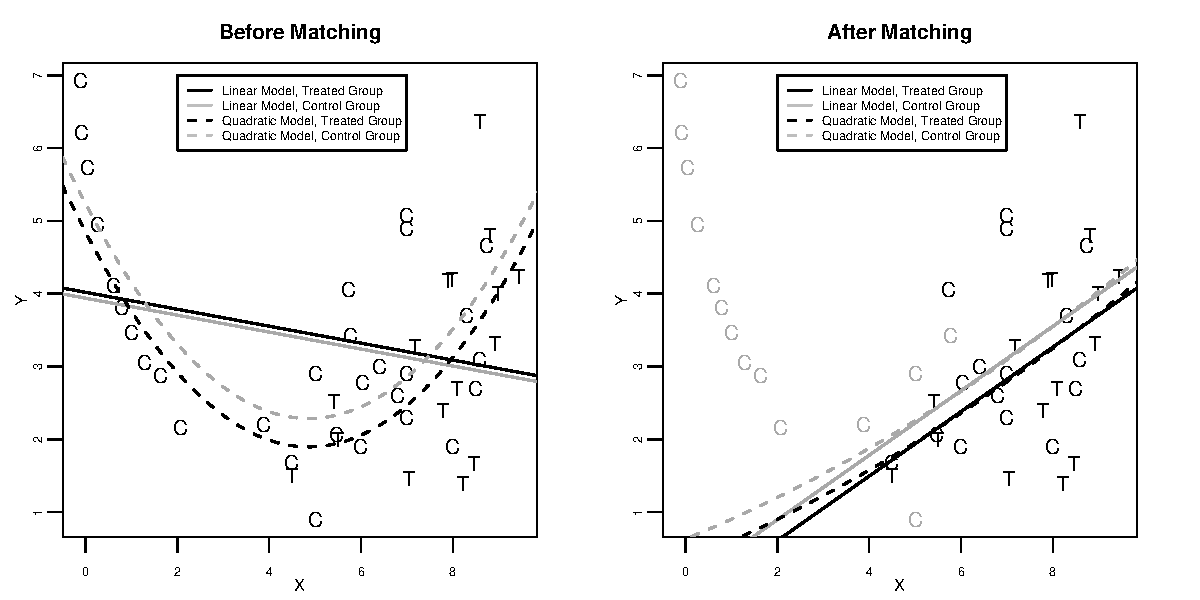
\includegraphics[width=6in]{figs/olspanel-thick.pdf}
  \end{center}
  \vspace{-0.275in}
  \caption{Model sensitivity of average treatment effect estimates for
    imbalanced raw and balanced matched data.  This figure presents an
    artificial data set of treated units represented by ``T'' and
    control units represented by ``C.'' The vertical axis plots $Y$
    and the horizontal axis plots $X$.  The panels depict estimates of
    the average treatment effect for a linear and quadratic
    specification, represented by the difference between parallel
    lines and parabolas, respectively.  Dark lines are fitted to the
    treated points and gray to the controls.  In the raw data, plotted
    in the left panel, some of the control units are far outside the
    range of the treated units, and these outlying control units are
    influential in the parametric models.  In the matched data,
    plotted in the right panel, treated units are matched with control
    units that are close in $X$ (gray units are discarded) and as a
    result treatment effect estimates are similar regardless of model
    specification.}
  \label{fg:extrap}
\end{figure}

Model dependence is easy to see by also fitting a quadratic model to
the same data, which merely involves adding an $X^2$ term to the
original linear regression.  Fitted values for the quadratic
regression appear as dashed curves in the same left graph, again gray
for the controls and solid black for the treated.  Clearly, these fit
the same data markedly differently from the original regression.  Not
only is the overall shape completely different, but the causal effect
has now switched signs, which can be seen because the gray solid line
is \emph{below} the dark solid line, whereas the gray dashed curve is
\emph{above} the dark dashed curve.

Ultimately, these two models estimate the causal effect by the average
vertical distance between the C's and T's.  They differ only in how
they compute this average.  In this case, the linear model estimates a
causal effect of $0.05$, while the quadratic model estimates a causal
effect of $-0.04$, and of course other models would yield other
estimates.  A key problem that generates this model dependence is the
presence of control units far outside the range of the treated units.
The model estimation thus extrapolates over a range of data that does
not include treated and control units, and so is particularly
sensitive to the set of control units who do not look similar to the
treated units.  These extrapolations make causal effect estimates
exquisitely sensitive to minor modifications in the statistical model
\citep{KinZen06a}.

Some researchers surely respond to this diversity of possible models
by inadvertently choosing specifications that support their favored
hypotheses.  Current best practice is to portray forthrightly at least
some aspects of specification uncertainty in published work by giving
results for multiple specifications and evaluating how model-dependent
the substantive results are.  But researchers of course do not often
go very far in portraying the sensitivity of their causal inferences
to model specification, and conveying all the sensitivity is
essentially impossible.  Indeed, attempts to do so in many situations
lead to nihilistic conclusions.\footnote{Two approaches to this
  problem include extreme bounds analysis \citep{Leamer78}, which is a
  somewhat standardized way to portray model dependence, and Bayesian
  model averaging \citep{HoeMadRaf99,ImaKin04}, which is intended to
  draw inferences by appropriately combining inferences from models
  with different specifications.}

\section{Nonparametric Preprocessing} \label{s:nonparpreproc}

The goal of matching in general and our specific nonparametric
preprocessing approach in particular is to adjust the data prior to
the parametric analysis so that (1) the relationship between $t_i$ and
$X_i$ is eliminated or reduced, and (2) little bias and inefficiency
is induced.  If we are able to adjust the data so that $t_i$ and $X_i$
are completely unrelated (which makes the control and treatment groups
identical with respect to $X$), we will have moved a good deal of the
way from Section~\ref{s:paraobs} to Section~\ref{s:paraexp}.  An
assumption of ignorability is still necessary, but we would no longer
need to model the full parametric relationship between the dependent
variable and the multidimensional $X_i$.  This also eliminates an
important source of model dependence in the resulting parametric
analysis stemming from the functional form specification and the curse
of dimensionality.  For data sets where preprocessing reduces the
extent of the relationship between $t_i$ and $X_i$, but is unable to
make them completely independent, model dependence is not eliminated
but will normally be greatly reduced.  If nonparametric preprocessing
results in no reduction of model dependence, then it is likely that
the data have little information to support causal inferences by
\emph{any} method, which of course would also be useful information.

But how can we adjust the data without inducing bias in our causal
estimates?  The key to this problem is that the fundamental rule for
avoiding selection bias --- not selecting on the dependent variable
--- does not prevent us from selecting observations on the explanatory
variables ($t_i$ or $X_i$).  (Random or other physical assignments
that depend on observed covariates, such as matched pair or randomized
block designs, in experiments and stratified sampling in surveys are
other examples of valid data collection mechanisms that select
observations given chosen values of the explanatory variables.)  We
can also select, duplicate, or selectively drop observations from an
existing sample without bias, as long as we do so using a rule that is
a function only of $t_i$ and $X_i$.  Our preprocessed dataset will
therefore include a selected subset of the observed sample for which
$t_i$ and $X_i$ are unrelated, meaning that the treatment and control
groups have the same background characteristics, or in other words
that this relationship holds:
\begin{equation}
  \label{balance}
  \tilde p(X\mid t=1) = \tilde p(X\mid t=0),
\end{equation}
where $\tilde p$ refers to the observed empirical density of the data,
rather than a population density.\footnote{To be more specific, the
  empirical density is defined as $\tilde p(x) = \# \{ i\in \{1, 2,
  \dots, n \}: X_i = x \} / n$, for all $x$, where $\#\{a\}$ is the
  number of elements in the set $\{a\}$.  The denominator in
  (\ref{balance}) is $\sum_{i=1}^n t_i$ on the left side and
  $\sum_{i=1}^n (1-t_i)$ on the right.}  The simplest way to satisfy
(\ref{balance}) by preprocessing is to use \emph{one-to-one exact
  matching}.  The idea is to match each treated unit with one control
unit for which all the values of $X_i$ are identical.  Our
preprocessed dataset thus is the same as the original dataset with any
unmatched units discarded, and thus with $t_i$ and $X_i$ now
independent.  If enough matches are available, this procedure
eliminates all dependence on the functional form in the parametric
analysis.  It is also highly intuitive, since it directly parallels an
experiment where we find pairs of units that are identical in all
observable ways and assign one from each pair to be treated and the
other to be a control.  Then no matter what effect $X_i$ has on $y$,
we can ignore it entirely since $X_i$ is literally held constant
within each pair of units.\footnote{Formally, ignorability (by which
  we mean the independence of $t$ and the potential outcomes given
  $X$) and balance (i.e., Equation \ref{balance}) guarantee valid
  inferences.  Together they are written as $p(Y(0)\mid
  t=1,X)=p(Y(0)\mid t=0,X)$ and $p(Y(1)\mid t=1,X)=p(Y(1)\mid
  t=0,X)$.}

Although one-to-one exact matching can eliminate model dependence and
any bias from incorrect assumptions made during the parametric stage
of analysis, it is not the only way to break the link between $t$ and
$X$, since satisfying (\ref{balance}) only requires the distributions
to be equivalent.  Moreover, exact matching has the disadvantage in
many data sets of not generating many matches.  The problem is most
severe if $X_i$ is high dimensional (another effect of the curse of
dimensionality) or contains continuous variables.  The result may then
be a preprocessed data set with very few observations that results in
a parametric analysis with large standard errors.  In this situation,
we may reduce model dependence and the potential for bias, but
decrease efficiency and as a result increase mean squared error.  If
this occurs, common practice is to sacrifice some bias reduction for
the increased efficiency that comes from having more observations in
the preprocessed dataset.  In our approach, if we lose some
opportunity for bias reduction we do so only in the preprocessing
stage; our second stage parametric analysis still has a chance to
eliminate the remaining bias.  This second chance does not apply if
only the difference in means is used.  We therefore turn in
Section~\ref{s:choose} to a menu of matching procedures that enable
researchers to satisfy (\ref{balance}) as closely as possible while
still generating a preprocessed dataset with enough observations.

We now offer an example, in the right graph in Figure~\ref{fg:extrap},
of the reduction in model dependence produced by matching that is not
exact.  The data in this panel is the same as that for which the
parametric analyses in the left graph gives highly model-dependent
results.  The difference is that the matching procedure deleted the
observations that would require substantial extrapolation (marked as
gray C's) and produces imbalance.  With these deletions, the data set
is now highly balanced, and as such the linear model and the quadratic
model give essentially identical causal effects.  In the matched data,
both parametric models yield estimates of approximately $0.001$ (which
is close to the true effect of $0$ we used to generate the data).
Preprocessing has therefore made the functional form assumption about
whether to include $X^2$ in the regression largely irrelevant.
Indeed, for a large range of models, this preprocessed data set will
be mostly insensitive to the choice of functional form assumptions and
so will return highly similar causal effect estimates.

A key point about matching as nonparametric preprocessing is that
matching is \emph{not} a method of estimation: obtaining causal effect
estimates from matching requires that it be paired with some analysis
method.  In the vast majority of applications, the analysis method has
been a simple difference in means between the treatment and control
groups.  This method certainly makes sense in the case of exact
one-to-one matching, since most parametric procedures applied to
exactly matched data would give the same estimates.  However, with
matching that is not exact, using a difference in means test is
equivalent to assuming that any remaining imbalance in the matched
sample is strictly unrelated to the treatment, which we know is false,
or has no effect on the outcome, which we have no evidence about
before consulting the outcome variable, and we will often have good
evidence to the contrary in real analyses.  For the same reason
scholars rarely use an unadjusted difference in means to analyze
randomized data, they should not use it in inexact matched data.
Thus, we recommend that scholars make use of our decades of experience
with parametric models to adjust (i.e., to interpolate or extrapolate)
the matched sample.  The adjustment necessary is far less onerous,
model dependent, and thus much more empirical than what would be
necessary without matching.

Finally, we note two advantages of our general framework. First, our
two-step procedure is ``doubly robust'' in the sense that if
\emph{either} the matching \emph{or} the parametric model is right,
causal estimates will be statistically consistent
\citep[see][]{RobRot01}.  That is, if the parametric model is
misspecified, but the matching is correct, or if the matching is
inadequate or wrong but the parametric model is correctly specified,
then our estimates will still be consistent.  The double robustness
property does not apply generally to using matching with a difference
in means.  Second, matching can improve efficiency of subsequent
parametric analyses while reducing the bias. Efficiency gain occurs
when matching reduces heterogeneity in the data by keeping only those
observations that are similar to each other and as a result helps
parametric models fit better, or more directly by removing the
dependency between the treatment variable and covariates.  To see
this, consider a simple linear regression with one treatment variable,
$T$, and one covariate, $X$.  The variance of the coefficient for the
treatment variable is equal to $\sigma^2/[n (1-\gamma) s^2_T]$ where
$\sigma^2$ is the conditional variance of the dependent variable, $n$
is the number of observations, $s^2_T$ is the sample variance of the
treatment variable, and $\gamma$ is the regression coefficient of $X$
on $T$. If matching reduces heterogeneity, then $\sigma^2$ will become
smaller.  If matching reduces the dependence between $T$ and $X$, as
is the goal in reducing bias, then $\gamma$ will be close to zero.
Then, the resulting variance for the treatment effect may become
smaller even if some observations are dropped and $n$ becomes smaller.
This suggests that so long as one keeps as many observations as
possible, matching might well often be able to reduce bias and improve
the efficiency of subsequent parametric analyses.

\section{Practical Implications of the Theoretical Matching
  Literature}
\label{s:choose}

In this section, we organize the practical information available in
the largely theoretical statistics, economics, epidemiology, medical,
and biostatistics literatures on matching.  We give special attention
to important instances where the theoretical literature has been
misunderstood by applied researchers and others across fields.  (For
technical literature reviews, see \citet{Imbens04},
\citet{Rosenbaum02}, and \citet{Stuart04} and the detailed user's
guide to the software that accompanies this paper; see Appendix
\ref{s:matchit}).

The goal of matching is to improve \emph{balance}, the degree to which
the treatment and control $X$ distributions resemble each other,
without losing too many observations in the process.  The main
diagnostic of success is also balance, the specific details of which
we describe below, as well as the number of observations remaining
after matching.  In seeking better balance, one can try any number of
matching procedures, and choose the one with the best balance as the
final preprocessed data set.  To ensure that selection during
preprocessing depends only on $X$ (to prevent inducing bias), the
outcome variable $y$ should not be examined during the preprocessing
stage.  As long as $y$ is not consulted, preprocessing cannot result
in stacking the deck one way or another.  Experimenters typically
follow a similar procedure by repeating randomization as often as
desired before collecting the outcome data; if an undesirable
randomization is obtained, such as with all men in the treated group
and all women in the control group, they merely discard the first
randomization and do it again until better balance is obtained
\citep[see][]{Rubin01}.

We discuss four aspects of preprocessing, followed by standard
parametric modeling of the preprocessed data set.  We describe this
procedure for the ATT, so the matching is designed to choose control
units that look most like the treated units.

\paragraph{Selecting Covariates}
All variables in $X$ that would have been included in a parametric
model without preprocessing should be included in the matching
procedure.  By the usual rules for avoiding omitted variable bias
these should include all variables that affect both the treatment
assignment and, controlling for the treatment, the dependent variable.
To avoid post-treatment bias, we should exclude variables affected by
the treatment.  

The theoretical literature emphasizes that including variables only
weakly related to treatment assignment usually reduces bias more than
it will increase variance \citep{RubTho96, HecIchSmi98}, and so most
believe that all available control variables should always be
included.  However, the theoretical literature has focused primarily
on the case where the pool of potential control units is considerably
larger than the set of treated units.  Applied researchers seem to
have incorrectly generalized this advice to all data sets.  If, as is
often the case, the pool of potential controls is not much larger than
the pool of treated units, then always including all available
controls is bad advice.  Instead, the familiar econometric rules apply
about the tradeoff between the bias of excluding relevant variables
and the inefficiency of including irrelevant ones: researchers should
not include every pre-treatment explanatory variable available.

\paragraph{Common Support Problems}

Finding balance is traditionally broken into two components: ensuring
\emph{common support} by pruning observations where the empirical
density of the control units and that for the treated units do not
overlap and additional selection (or later adjustment) to make the
portions of the densities that do overlap have the same heights.
Areas outside of common support are particularly problematic since
they require extrapolation, which can generate considerable model
dependence.  And indeed the farther the extrapolation is from the data
the larger can be the model dependence.  For example, asking in 2001,
what Iraq would be like if the U.S.\ attempted to impose democracy
there, was pure extrapolation since the U.S.\ had not previously
attempted the same thing in another country like Iraq in all relevant
respects.  Making such an inference could only be made on the basis of
theoretical modeling assumptions because relevant empirical
observations from the control group do not exist.

In the applied literature, researchers often skip this step, which can
be a major mistake.\footnote{Some try to find common support by using
  the ``propensity score,'' which we describe below.  This approach
  may not be appropriate, however, since the propensity score can only
  be used to to find common support when it is validated, but
  validation cannot occur when the data include observations outside
  common support \citep[see][and the discussion below]{KinZen06a}.}
After all, balance can always be improved and potential model
dependence reduced by removing units that require extrapolation.  Part
of the reason this step is skipped so often is that it has not until
recently been clear how to identify units that require extrapolation.
One easy approach, developed by \citet{KinZen06a} is to prune
observations from the control group that are outside of the ``convex
hull'' of the treatment group.  With one pre-treatment covariate, the
convex hull of the treatment group is merely the range of the subset
of observations of $X$ that are in the treatment group (because
$t_i=1$), so control units greater than max($X$) or less than min($X$)
are discarded.  The general definition of the convex hull (which is
more sophisticated than the range in multiple dimensions) also works
to define regions of extrapolation with any number of
covariates.\footnote{Similarly, if any treated units fall outside the
  convex hull of the control units, these too are often discarded.
  Dropping treated units changes the causal effect being estimated,
  and so should be done with more caution, but if it remains a
  relevant quantity of interest, at least it can be estimated in a
  reasonable way.}  Across this and the other methods of checking
common support, the more conservative the approach that defines common
support more restrictively, the less model dependence.  Of course,
more conservative approaches also leave fewer observations.

\paragraph{Exact Matching}  
It is always worth checking to see whether each treated unit can be
matched to all control units with exactly the same covariate values.
This procedure is more general than the more commonly tried one-to-one
exact matching, since we use as many control units as are available
for each treated unit.  If a large number of units were matched, then
we have exact balance with little inefficiency and we may skip the
remaining steps.  Indeed, exact balance means that a difference in
means is sufficient for the parametric analysis (but be sure to
compute a difference in weighted means if very different numbers of
matches are included for each unit).  If an insufficient number of
matches is found, we either repeat the exact matching with fewer
covariates or switch to other methods, described below.  In the
former, we balance the included variables but do not balance at all on
the rest.  The excluded variables may be partially balanced due to
correlations with the included variables, but some balance will be
absent.  In contrast, other methods, such as propensity score
matching, use all variables but only approximately matches.

\paragraph{The Propensity Score Tautology}
A commonly used matching procedure is to summarize all the variables
in $X$ with a single variable called the \emph{propensity score}
\citep{RosRub83}.  The propensity score is the true probability of
unit $i$ receiving treatment, given the covariates $X_i$, $e_i(X_i) =
p(t_i=1 | X_i)$.  It is usually estimated via a logistic regression of
$t_i$ on a constant term and $X_i$ (without regard to $y$).
Unfortunately, the role of the propensity score in the theoretical
literature differs profoundly from the way it has been widely used in
practice.  Understanding this disconnect, an explanation of which to
our knowledge has not explicitly appeared before in the literature, is
fundamental to making good practical use of this important concept.

Theoretically, the true propensity score is valuable because it is a
``balancing score,'' meaning that if a group of units have identical
propensity score distributions, then all the covariates will be
balanced in the treated and control groups.  In addition, if treatment
assignment is strongly ignorable given the covariates $X$, then it is
also ignorable given only the propensity score.  This means that
matching can be done using just the one-dimensional propensity score,
instead of all of the variables in $X$.  Using the true propensity
score in this way, as does much of the applied literature, would thus
apparently solve the curse of dimensionality for matching.

In practice, however, we do not know the \emph{true} propensity score
(except in unusual situations like experiments).  We would still be
able to appeal to some of the true propensity score's theoretical
properties if we had a consistent estimate of it, but such an estimate
would require knowing the correct functional form for the assignment
model, which is highly unlikely.  Moreover, few useful theoretical
results exist for the case when the true form of the propensity score
equation remains unknown.  These theoretical results would therefore
seem to be entirely self-defeating: In order to use nonparametric
matching to avoid parametric modeling assumptions, we must know the
parametric functional form of the propensity score equation!

Fortunately, there is a way out.  We suggest, first, looking past the
theoretical properties of the propensity score, except for the purpose
of motivating the goal of better propensity score specification, and
second and more importantly, recognizing the value of what we call the
\emph{propensity score tautology}.  The propensity score tautology in
our view is the main justification for using this technology in
practice: The estimated propensity score is a balancing score when we
have a consistent estimate of the true propensity score.  We know we
have a consistent estimate of the propensity score when matching on
the propensity score balances the raw covariates.  Of course, once we
have balance on the covariates, we're done and don't need to look
back.  That is, it works when it works, and when it doesn't work, it
doesn't work (and when it doesn't work, keep working at it).

The tautology thus provides a way to make irrelevant the knowledge of
whether we have satisfied the conditions necessary to use the
theoretical results about the true or consistently estimated score.
The goal of matching is to achieve the best balance for a large number
of observations, using any method of matching that is a function of
$X$, so long as we do not consult $y$.  As it turns out, and for
whatever reason, one such method that researchers sometimes find
useful in some applications is based on propensity scores.  The reason
the propensity score approach often works in practice to balance the
covariates relatively quickly may be related to its as yet unproven
theoretical properties, but this conjecture is irrelevant to making
valid causal inferences.  At least given the current state of the
literature, only the propensity score tautology is useful in practice.
Other theoretical results have no direct bearing on practice.

In applications, the usual practice is to estimate the propensity
score by a logistic regression of $t_i$ on $X_i$.  Since we are in the
situation where exact matching is insufficient, a common procedure is to
match each treated unit to the control unit with the most similar
value of the estimated propensity score $\hat{e}_i$ (which is known as
nearest neighbor matching on the propensity score).\footnote{When
  matching without replacement, two different approaches of matching
  nearest neighbors are available. The first, known as ``greedy''
  matching, starts with some treated unit and matches the closest
  control unit that has not yet been matched.  This approach, although
  slightly faster and easier to understand, is not invariant to the
  order in which units are matched.  A second approach, known as
  ``optimal'' matching, avoids these issues by minimizing the total
  distance within matched units \citep[e.g.,][]{Rosenbaum89}.  Our
  software implements both, incorporating optimal matching code
  provided by \citet{Hansen04}.}  If this procedure balances $X$ (and
thus satisfies the procedures for checking balance we describe below),
we use it.  If not, then we respecify the logistic regression by
adding interactions or squared terms and match again.  If that works,
then we use it.  If not, we try even more elaborate specifications
(such as other functional forms such as CART, neural network analyses,
or others) or more sophisticated matching methods
\citep{Frolich04,SmiTod05}.

\paragraph{Deciding Which Observations to Match}
The collective wisdom of the literature recommends the following three
procedures for the actual process of choosing matched data sets.
First, if many more control than treatment units are available,
choosing more than one control match for each treated unit will
increase the efficiency of the procedure (although each match past the
first usually reduces the variance less than the previous one), and
can in some instances greatly reduce the bias too \citep{Smith97}.
If, instead, fewer controls are available than those treated, then
matching with replacement --- allowing each control unit to be matched
to more than one treated unit --- is a good option \citep{DehWah99}.
Alternatively, we can consider switching the definition of treatment
and control groups (although, if using ATT, this will change the
substantive definition of the causal effect unless one uses more
sophisticated estimators; \citealt{Lechner00}).

Second, we are sometimes in the situation of suspecting from prior
evidence (but not from the present data set) that a small number of
covariates have a disproportionately large effect on our outcome
variable.  When this is the case, even slightly mismatching on these
variables may severely bias our causal effect.  To avoid this problem,
we suggest matching using two separate metrics, one for the
large-effect variables and another for the rest.  If feasible, we
create pools of exact matches on the large-effect variables and then
use nearest neighbor matching based on the remaining variables to
choose specific matches within these pools.  If exact matching does
not turn up sufficient observations, then we can choose the nearest
neighbor on the large-effect variables, defined by the Mahalanobis
distance, among all units within say 0.25 standard deviations (also
known as ``calipers'') of the propensity score computed from all
variables.\footnote{The 0.25 standard deviation figure, although not a
  universal constant of nature, is the most common recommendation in
  the literature; it appears to have been interpolated from the
  results in \citet{CocRub73}.  The Mahalanobis distance is the
  weighted average of the squared distance between units $i$ and $j$,
  $(X_i-X_j)'\Sigma^{-1}(X_i-X_j)$, where $\Sigma$ is the sample
  covariance matrix of $X$ in the control group.  See
  \cite{RubTho00}.}  If some of the variables in $X$ represent binary
variables with very few in one category, common practice is to include
them in the propensity score but not in the Mahalanobis distance
calculation (\citealp{GuRos93, RubTho00}).

Finally, if finding a matching procedure with good balance and a large
number of observations is difficult, subclassification can be a useful
technique.  In subclassification, we form groups in which the
distributions of covariates is the same, even though across the
subclasses the distributions of covariates may be quite different.
Subclassification can be accomplished by dividing the units into
roughly equally sized subclasses where the estimated propensity score
is, by construction, approximately constant, and thus balanced.  Many
rely on the theoretical result that five or six subclasses are
sufficient to adjust for a univariate covariate such as the propensity
score \citep{Cochran68,RosRub84}, but applied researchers have not
fully appreciated that as $n$ increases more subclasses are generally
preferable.  In addition, the number and definition of the subclasses
should be tuned to the nature of the empirical distributions to ensure
adequate treatment and control units in each subclass.  A useful
alternative is ``full matching'' methods, which offer variable numbers
of matches in each subclass \citep{Hansen04}.

\paragraph{The Balance Test Fallacy}

A good matching procedure reduces bias by increasing balance, does not
increase the variance much, and prevents inducing new biases by
matching only based on $X$ without consulting $y$ until the analysis
stage.  We assume matching is based only on $X$, and checking the
number of observations remaining after matching is easy.  Thus, the
main issue we address in this section and the next is how to evaluate
balance.  Conceptually, verifying balance involves checking whether
(\ref{balance}), $\tilde p(X|t=1)=\tilde p(X|t=0)$, holds.  One way to
think about this process is to imagine, for all the variables in $X$,
forming a multidimensional histogram for all the treated units and
comparing it to another multidimensional histogram of all the control
units.  Because of the curse of dimensionality, multidimensional
histograms with more than a few covariates tend to be very coarse or
have many empty bins, and so using them to estimate the two underlying
probability densities in (\ref{balance}) will ordinarily be very
difficult without access to an extraordinary number of observations.
Thus researchers usually examine various low dimensional summaries
instead.  If a low dimensional summary differs between the treated and
control groups then (\ref{balance}) does not hold.  The risk of course
is that even if the treatment and control groups match according to
some low dimensional summaries, we still cannot be certain that
(\ref{balance}) holds since it is a multivariate concept, and so using
several different checks is always a good idea.

Here we describe what we call the balance test fallacy, which
unfortunately characterizes most applications of matching in most
fields.  The critical misunderstood point is that balance is a
characteristic of the observed sample, not some hypothetical
population.  The idea that hypothesis tests are useful for checking
balance is therefore incorrect, and t-statistics below 2 and p-values
above 0.05 have no special relevance for assessing balance.

The fallacy has several serious implications.  First, balance tests do
not provide levels below which imbalance can be ignored: The closer
the two observed treatment and control groups in the sample, the
better.  Even though we might use a hypothetical population that
generates the observed $X$ to think about concepts like common
support, it is the observed sample that is relevant for generating
balance.  To see this, consider in assessing the effect of some
treatment whether we want the treatment and control groups to be
identical, or whether we should be willing to risk them being slightly
different.  The problem that has been ignored is that if the
difference, no matter how small, occurs for a variable that happens to
have a large enough effect on $Y$, then this tiny or ``insignificant''
imbalance can translate into a large bias and/or inefficiency in our
causal estimates.

The balance test fallacy has led hypothesis tests to be used
extensively in applications of matching.  Most commonly, tables of
t-tests for differences in means are offered as evidence that balance
has been ``achieved''.  This is unfortunate since a better balanced
sample, that would reduce bias even further, can often be found.  But
even more importantly, hypothesis tests not only can cause one to stop
too soon, but they can be highly misleading even when using them as
objective functions to optimize.  In particular, pruning too many
observations reduces the statistical power of a hypothesis test (i.e., the
probability of rejecting the null hypothesis) and thus affects the
test, even if this pruning does not improve balance at all.

\begin{figure}[t] 
 \begin{center}
   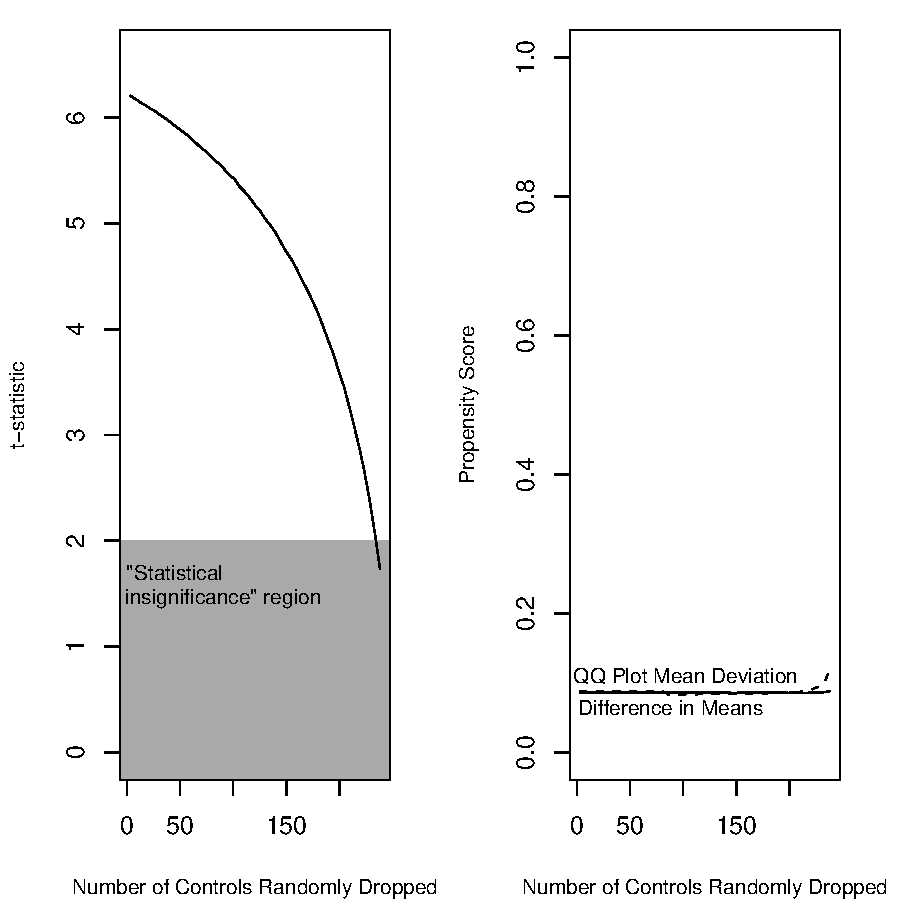
\includegraphics[height=4in]{figs/TStatPlotPscore.pdf}
  \end{center}
  \vspace{-0.275in}
  \caption{Dangers in relying on t-statistics as measure of balance.
    The solid lines in both graphs indicate the average value of a
    measure of balance when a given number of control units are
    randomly dropped from the data set (out of a total of 245).  With
    larger numbers of control units dropped (i.e., smaller numbers of
    control units in the resulting sample), the t-statistic gets
    closer to 0, falsely indicating reductions in balance with the
    smaller resulting sample sizes, even though true balance does not
    vary systematically across the data sets.}
  \label{f:tstat}
\end{figure}

To illustrate the dangers of using hypothesis tests to assess balance,
we created a sequence of matched data sets by \emph{randomly} pruning
increasing numbers of control group observations (from the real data
set we analyze in Section~\ref{s:carp}).  Random matching procedures
have no systematic effect on balance.  Yet, the left graph in
Figure~\ref{f:tstat}, which plots the number of observations dropped
(plotted horizontally) by the t-statistic (plotted vertically), shows
that the t-statistic falsely indicates a dramatic improvement in
balance.  The area where the t-statistic falls below 2 is normally
(but incorrectly) identified as ``insignificant imbalance,'' and
clearly the t-statistic drops into this area (colored grey in the
figure) only because of the sample size and regardless of the fact
that the balance does not differ systematically as more observations
are dropped.  In fact, since hypothesis test are driven in part by
factors other than balance, they are not even monotonic functions of
balance: the t-test can get apparently better while balance gets
worse, or vice versa.\footnote{To see this, consider the commonly-used
  two sample $t$-test statistic with unknown and unequal variances,
  which can be written as, $\sqrt{n}(\overline{X}_t-\overline{X}_c)/
  \sqrt{\frac{s^2_t}{r} + \frac{s^2_c}{1-r}}$ where
  $s^2_t=\sum_{i=1}^n t_i(X_i - \overline{X}_t)^2/(n_t-1)$,
  $s^2_c=\sum_{i=1}^n (1-t_i)(X_i - \overline{X}_t)^2/(n_c-1)$, $n_t$
  and $n_c$ are the sample size for the treatment and control groups,
  and $r=n_t/n$.  Hence, the difference in sample means as a measure
  of balance is thus distorted in the t-test due to the three factors:
  the total number of remaining observations $n$, the ratio of
  remaining treated units to the total number of remaining
  observations $r$, and the variance of $X$ for the remaining treated
  and control units, $s_t^2$ and $s_c^2$ respectively.}

\paragraph{Better Matching Evaluations}

Instead of using hypothesis tests for assessing balance, we need to
assess the difference in the multivariate empirical densities of $X$
for the treatment and control groups.  Since working with multivariate
densities is difficult, we follow the common procedure of working with
lower dimensional summaries, but we do so by directly assessing
differences.  We also recommend that the measures applied be presented
in the units of the original variables, so that the substance of the
problem is emphasized and the relationship between the size of the
remaining imbalance can be compared to one's views about the potential
importance of the variable in question.

One particularly simple low dimensional summary compares the mean of
each variable in $X$ for the treated group with the mean of each
variable in the control group.  The smaller these are the better.  One
rule of thumb that has been offered is if one or more of these differ
by more than half a standard deviation of the respective $X$ variable,
then better balance is needed \citep{Cochran68}, but finding ``small''
imbalance in the original units is the real goal.  It is also useful
to compare the standard deviations of each variable between the two
groups, as well as interactions or higher order moments.  Another
useful procedure is to compare treatment and control histograms one
variable at a time or in pairs if enough data are available.

Our preferred approach is to use an empirical quantile-quantile plot,
or QQ-plot, for each variable (and often their interactions) to
compare the distributions of the full densities for the treated and
control groups for each variable.  QQ-plots are usually the best way
to compare two univariate distributions: They plot the quantiles of a
variable of the treatment group against that of the control group in a
square plot (we give examples in Section \ref{s:emp}).  We also
numerically summarize these plots with mean and maximum deviation
between the two distributions on the scale of the variables being
measured (which is the average or maximum deviation from the 45 degree
line).\footnote{For example, the maximum distance of quantile
  functions, is given by $\max_{0 < \alpha < 1}
  |\widetilde{F}_{Xt}^{-1}(\alpha)-\widetilde{F}^{-1}_{Xc}(\alpha)|$
  where $\widetilde{F}_{Xt}$ and $\widetilde{F}_{Xc}$ are the
  empirical cumulative probability distribution functions of a single
  variable $X$ for the matched treatment and matched control groups,
  respectively. That is, $\widetilde{F}_{Xt}(x)=\frac{1}{n^*_t}
  \sum_{i=1}^{n^*} {\rm I}_{\{X_i \le x\}} t_i$ and
  $\widetilde{F}_{Xc}(x)=\frac{1}{n^*_c} \sum_{i=1}^{n^*} {\rm
    I}_{\{X_i \le x\}} (1-t_i)$ where $n^*_t=\sum_{i=1}^{n^*} t_i$ and
  $n^*_c=\sum_{i=1}^{n^*} (1-t_i)$ are the size of matched treatment
  and matched control groups, $n^*=n^*_t + n^*_c$ is the size of
  matched data, and ${\rm I}$ denotes the indicator function.} (If one
wishes to compare the balance across different covariate dimensions,
then differences in empirical cumulative distribution functions can be
used, instead.)

A paradoxical but sometimes useful procedure is to examine the QQ plot
of the propensity scores of the control and treated units.  This is
paradoxical (and part of the propensity score tautology) because it
relies on the propensity score as a summary of the data to check
whether propensity score matching is adequate.  It is useful
nonetheless as one of our procedures for checking balance because it
offers a low dimensional summary not obviously worse than 
examining the variables one at a time.  Indeed, for the reasons discussed
above, it is often a good low dimensional summary.

The immediate goal of matching is balance, which involves adjusting
the data set to reduce dependence between $t$ and $X$.  Since for
feasibility scholars will use one dimensional summaries to substitute
for the comparison of multidimensional histograms, evaluating balance
should always be done in multiple ways.  Relying on any one measure to
assess balance will never be adequate (unless matching is exact).  In
addition, the ultimate goal of matching is not merely balance, but
reducing bias and model dependence in estimating the causal effect of
$t$ on $Y$.  We exclude any information from $Y$ in the matching
procedure so as to avoid selection bias, but the key is that causal
estimation bias and model dependence is a function of both imbalance
in our covariates \emph{and} our best prior information about the
importance of each covariate (the effect of $X$ on $Y$ controlling for
$t$).  Obtaining good balance on covariates that are likely to be
important is more crucial than those that have less of an effect since
important covariates will inflate any remaining imbalance to produce
more model dependence.  Thus obtaining a good matched data set
requires careful assessment and evaluation through multiple objective
functions (none of which involve balance hypothesis tests), as well as
the combination of the quantitative measures discussed above and
available prior information about the likely relative importance of
each of one's covariates.  So long as balance is assessed by the same
standards, automated searches, such as the promising approach of
\citet{DiaSek05} (also incorporated in MatchIt), can also be useful in
finding good matches to evaluate.

If some covariates are omitted from some of the matching procedures,
the balance on them should still be checked.  Doing so is often a good
way to discover important covariates, since in fact researchers
frequently have good qualitative knowledge of variables not coded in
$X$, especially in nonsurvey data on countries or regions
\citep[][Ch.3]{Rosenbaum02}.  Indeed, preprocessing can help
researchers better understand their data when supplemented by good
qualitative information and research \citep[e.g.,][]{RosSil01}.

If meeting these criteria for balance proves impossible, we then need
to recognize that preprocessing by matching may not be helpful.
Unfortunately, if preprocessing is unhelpful, then any parametric
procedure will likely require severe extrapolation and hence will be
highly model-dependent.  In the unusual situation where particular
parametric assumptions are somehow justified and verified, then it may
be reasonable to proceed.  In most applications, however, model
sensitivity that cannot be improved by preprocessing because balance
is too hard to achieve marks a data set that is too fragile for making
robust causal inferences by any means.

% The power function is given by $$
% T_{n'_t+n'_c-1}(-c_{\alpha/2} \mid
% \phi) + 1-T_{n'_t+n'_c-1}(c_{\alpha/2} \mid \phi)$$
% where $T_\nu$ is
% the distribution function of $t$ distribution with $\nu$ degrees of
% freedom, $c_{\alpha/2}=T_{n'_t+n'_c-1}^{-1}(1-\alpha/2)$ and $$\phi =
% \frac{\mu_1-\mu_2}{\sigma\sqrt{\frac{1}{n'_t}+\frac{1}{n'_c}}}$$

\paragraph{Parametric Outcome Analysis}  
After choosing the final matched sample, preferably with maximum
balance and a large number of observations, the parametric analysis
can then proceed.  Unfortunately, with few exceptions the parametric
analysis chosen in practice by applied researchers after matching has
been a simple difference in means (or the equivalent of a regression
of $Y$ on $T$ without any control variables).  This is unfortunate,
since the procedure assumes that $T$ and $X$ are unrelated.  If the
assumption is false, and it is false except in the rare case when
exact matching is possible for all observations, then the result is
the same for omitted variable bias that occurs whenever a potential
confounding variable is ignored.

Thus, with one possible exception, a better procedure is to use the
same parametric analysis on the preprocessed data as would have been
used to analyze the original raw data set without preprocessing.  This
can include the same maximization algorithms, the same software, the
same model checking and fit procedures, and the same methods of
computing and interpreting quantities of interest.  The one exception
is that for subclassification, the parametric analysis should be
conducted separately within each subclass, and the results combined by
taking a weighted average (with weights based on the number of units
in each subclass), or, if insufficient observations exist within each
subclass, fit an overall model with fixed or random effects for the
subclasses.  Using preprocessed data should reduce model dependence,
and this too is worth checking: as one should even without
preprocessing, we should check the sensitivity of causal effect
estimates to changes in the specification.

\paragraph{Computing Uncertainty Estimates}

Computing uncertainty estimates, such as standard errors or confidence
intervals, from matching procedures is an active area of research
where no consensus yet exists.  The problem is not some disagreement
over technical statistical issues.  Rather, the issue revolves around
normative criteria such as what researchers should condition on and
what they should attribute to additional uncertainty.  Since scholars
are no more likely to reach consensus via debate on normative
statistical issues than on normative political issues, the best way
forward may be to choose a reasonable definition, show how to compute
uncertainty estimates for it, and let others pick different
definitions if they prefer.  Our choice, which we now explicate,
appears substantively reasonable and has the advantage of being easy
to implement.

Our idea is to take advantage of a common feature of all of the
methods of computing uncertainty estimates associated with parametric
methods: They are all conditional on the pretreatment variables $X$
(and $t$), which are therefore treated as fixed and
exogenous.\footnote{These include methods based on using the
  asymptotic normal approximation to the likelihood function, direct
  simulation from the finite sampling distribution or posterior
  density, various frequentist bias corrections, robust Bayesian
  analysis involving classes of posteriors, and even nonparametric
  bootstrapping, among others.}  Since our preprocessing procedures
modify the raw data only in ways that are solely a function of $X$, a
reasonable method for defining uncertainty is to continue to treat
$X$, and thus our entire preprocessing procedures, as fixed.  The
advantage of this definition is that we can easily compute standard
errors and confidence intervals using the same methods researchers
have been using with their parametric methods all along, but applied
to the preprocessed instead of raw data.  (The one exception to our
procedure occurs when matching with replacement, where we would then
run the parametric procedure with each unit weighted proportional to
the number of times it was chosen as a match.)  As proper procedures
are developed to include different aspects of matching in the
uncertainty estimates, these could be used also, but they would each
estimate a different variance quantity.

Thus, when estimating the ATT or ATE, we compute estimates of
$\mu_i(1)$ and $\mu_i(0)$ and their uncertainty as usual from the
parametric model applied to the preprocessed data.  If computing
conditional causal effects (either on average over all observations or
just the average for the treated units), we set $\mu_i(1)=y_i$ if
$t_i=1$, and use the parametric model to estimate $\mu_i(0)$ and its
uncertainty, whereas if $t_i=0$, we set $\mu_i(0)=y_i$ and use the
parametric model to estimate $\mu_i(1)$ and its uncertainty estimate.

\section{Empirical Illustrations}\label{s:emp}

We now offer two empirical illustrations of how preprocessing raw data
via nonparametric matching can reduce model dependence.  For
pedagogical reasons, and to save space, we use different methods of
checking balance via (\ref{balance}) in our two applications.

\subsection{Democratic Senate Majorities and FDA Drug Approval
  Time}\label{s:carp}

An influential article by \citet{Carpenter02} tests a key hypothesis
in the literature on institutional and partisan determinants of
regulatory policy by examining several determinants of new drug
approval times by the U.S.\ Food and Drug Administration (FDA).  Here,
we focus on the hypothesis that Democratic oversight of the FDA should
lead to slower approval of new drugs (p.495) and the specification of
Model 1 of Table 2 (p.499).

To test this hypothesis, Carpenter uses a lognormal survival model of
approval times regressed on several causal variables of political
oversight (median adjusted ADA scores for House and Senate Committees
as well as for House and Senate floors, Democratic Majority in House
and Senate, and Democratic Presidency) and 18 control variables
including clinical and epidemiology factors and firm
characteristics.\footnote{In the original paper, \citet{Carpenter02}
  uses a lognormal frailty model with a common (ungrouped) random
  effect.  For computational simplicity, we drop the random effect.
  This has small effects on the quantities we estimate, and no effect
  on our conclusions.}  The dataset consists of 408 new drugs reviewed
by the FDA, 262 of which were eventually approved.  The remaining 146
drug applications were still pending at the time of data collection
and hence are treated as right-censored observations.  (Inferences
from the censored observations are necessarily model-dependent by
design and so this aspect of the problem is not influenced by the
methods we introduce.)  Approval time is measured in months passed
from the submission of an application.

We focus on the causal effect of a Democratic majority in the Senate,
one of the seven oversight variables. In particular, we estimate the
in-sample (conditional) average treatment effect for the treated.
Carpenter's remaining six oversight variables are conceptually and
statistically highly related, and are in part consequences of a
Democratic Senate majority.  As such, we omit them to avoid
post-treatment bias.  Post-treatment bias may still exist in this
research design if other variables controlled for are consequences of
a Democratic Senate majority.  For example, if media coverage of a
particular disease is affected by Democratic control, bias would be
induced.  Although post-treatment bias is a critical issue in
accurately estimating causal effects, it would affect parametric
models with or without preprocessing and so is less relevant for our
present goal of reducing model dependence; we do not pursue it
further.

% We also assume the absence of autocorrelation (or interference among
% units).  In this application, this assumption means that the existence
% of a Democratic Senate majority when one drug is considered by the FDA
% has no affect on the approval time of another drug (after
% controlling for the existence of a Democratic Senate majority and
% other control variables at the time of approval of the second drug).
% This assumption seems reasonably applicable to these data.

In the original analysis, the reported coefficient for the Democratic
Senate majority variable is statistically significant at the 10\%
level but in the opposite direction of Carpenter's hypothesis.  For
our purposes this variable is of particular interest because
\citet[p.498]{Carpenter02} finds that ``[t]he coefficient estimate for
this variable [Democratic Senate majority] is not significant in other
regressions, and even switches sign when firm variables are added.''
We therefore examine whether the model sensitivity that prevented
Carpenter from drawing firm conclusions about the Democratic Senate
majority variable is reduced by preprocessing the data. 

To preprocess, we follow the recommendations described in
Section~\ref{s:choose}. We first check whether the control units are
within the convex hull of the treated units using the method developed
by \citet{KinZen06a}. The result of this analysis indicates that none
of the control units is in the convex hull. This lack of
common support explains in part why \citet{Carpenter02} finds the
results are highly model-dependent. To proceed, we estimate the
propensity score using logistic regression with all covariates as
linear predictors.  We then discard 15 control units and 2 treated
units that are outside of the common support of the estimated
propensity score. Finally, we conduct one-to-one nearest neighbor
propensity score matching (without replacement) while placing exact
restrictions on the six binary variables (whether primary indication
is lethal condition, acute condition, and/or results in
hospitalization; whether disease mainly affects men, women, and/or
children). We choose one-to-one matching rather than one-to-many
matching or full matching because our convex hull analysis indicates
that most of the observations are likely to be outside of the common
support.  This preprocessing procedure discards 102 units (10 treated
units and 92 control units) from the original sample that would have
required substantial, model-dependent extrapolations. The matched data
sets then consists of 306 observations.
\begin{table}[t]
\begin{center}
\setlength{\tabcolsep}{2pt}
\begin{tabular}{lrrrrrr}
\hline
\hline
 & \multicolumn{2}{c}{} 
 & \multicolumn{4}{c}{Empirical Quantile Measures} \\
 & \multicolumn{2}{c}{Mean Difference} 
 & \multicolumn{2}{c}{Mean Difference} 
 & \multicolumn{2}{c}{Max Difference} \\
Variable Names 
& imbal. & \%imprv.
& imbal. & \%imprv.  
& imbal. & \%imprv. \\
\hline
Estimated propensity score & 0.04 & 56.76 & 0.04 & 56.20 & 0.09 & 52.85 \\
{\bf Clinical/Epidemiological Variables} & \\
Incidence of primary indication & 0.07 & 19.91 & 0.07 & 12.53 & 0.50 & 80.11 \\
Primary indication is lethal condition & 0.00 & 100.00 & 0.00 & 100.00 & 0.00 & 100.00 \\
Death rate, primary indication & $-$0.00 & 99.90 & 0.01 & 71.26 & 0.29 & 86.56 \\
Primary indication is acute condition & 0.00 & 100.00 & 0.00 & 100.00 & 0.00 & 100.00 \\
Primary ind. results in hospitalization & 0.00 & 100.00 & 0.00 & 100.00 & 0.00 & 100.00 \\
Hospitalizations associated with indication & 0.13 & 2.56 & 0.15 & 5.91 & 3.01 & $-$1.37 \\
Disease mainly affects women & 0.00 & 100.00 & 0.00 & 100.00 & 0.00 & 100.00 \\
Disease mainly affects men & 0.00 & 100.00 & 0.00 & 100.00 & 0.00 & 100.00 \\
Disease mainly affects children & 0.00 & 100.00 & 0.00 & 100.00 & 0.00 & 100.00 \\
Orphan Drug & $-$0.01 & 51.21 & 0.01 & 57.39 & 1.00 & 0.00 \\
\multicolumn{3}{l}{\bf Disease Politics (Groups and Media) Variables} & \\
National and regional groups & $-$0.00 & 89.60 & 0.02 & 53.07 & 0.80 & 26.61 \\
Nightly TV news disease stories & $-$0.14 & $-$15.63 & 0.14 & $-$27.60 & 3.23 & $-$11.21 \\
Washington post disease stories & $-$0.13 & 49.06 & 0.14 & 42.33 & 1.68 & 8.84 \\
Days of Congressional hearings & $-$0.02 & 20.22 & 0.07 & 29.66 & 1.70 & 38.55 \\
Order of disease market entry & 0.05 & 34.02 & 0.23 & $-$17.66 & 1.00 & 16.67 \\
{\bf FDA Variable} & \\
CDER staff & $-$0.68 & 10.77 & 1.57 & 5.78 & 3.06 & 17.96 \\
\hline
\hline
\end{tabular}
\end{center}
\caption{Remaining covariate imbalance after matching for the FDA data. 
  The table presents three different measures of resulting imbalance
  after matching --- sample mean differences, and mean and maximum
  values of differences in empirical quantile functions --- as well as
  their percent balance improvement over the raw data.  In almost all
  dimensions and across three different measures, matching
  substantially improves balance.} \label{tb:fdabal}
\end{table}

Table~\ref{tb:fdabal} summarizes how preprocessing can improve the
covariate balance. The table presents three balance measures after
matching for each covariate and their percent improvement as
compared to the original balance before matching.  Matching
substantially improves the balance of each covariate. Exact
restrictions with six binary variables make their balance perfect,
which is indicated by the fact that the values of all the balance
measures are zero and their percent improvements are 100.  Mean
differences are considerably smaller for all but one covariate;
empirical quantile measures also indicate a large improvement in
balance for most variables.  Preprocessing slightly increases the
values of empirical quantile measures in two cases.  Uniform
improvement of balance for all covariates and all measures is unlikely
unless exact matching is possible for all covariates. In this
particular example, the lack of common support in the original data
makes matching more difficult.  Therefore, we adjust the minor sample
differences that remain by fitting the parametric models to the
preprocessed data. By choosing the matched set of control units which
look most similar to the treated units, the treated-control comparison
will then take place only among units similar on the background
variables and thus will not be affected as much by the model
specification.

We now run the same log-normal survival analysis as Carpenter but
using the preprocessed data set.  Since nothing changed other than the
removal of observations that would have required highly
model-dependent inferences, no other analysis procedures change.  We
compute maximum likelihood estimates, standard errors, and confidence
intervals using the same procedures Carpenter did on the raw data.  By
applying this procedure to the preprocessed data, the estimated
average treatment effect for the treated based on Carpenter's Model 1
is approximately $-33.5$ months with an estimated standard error
of $7.5$, indicating that a Democratic Senate majority significantly
decreases the average approval time of new drugs.  This result thus
continues to contradict Carpenter's initial hypothesis.

Although data analysis would end here for those interested in the
substantive research question at hand, for our methodological purposes
we go a step further to study model-dependence.  For simplicity, we
portray model dependence by the variability in maximum likelihood
estimates of conditional in-sample ATT estimates across different
specifications of pretreatment covariates, although the same
conclusions apply to most other quantities of interest too.
\begin{figure}[t] 
 \begin{center}
   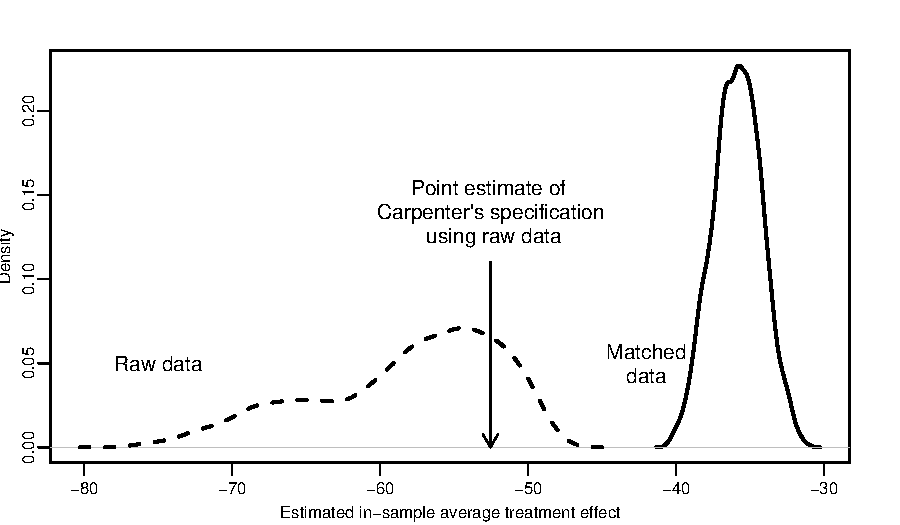
\includegraphics{figs/fdadens.pdf}
  \end{center}
  \vspace{-0.15in}
  \caption{Kernel density plot (a smoothed histogram) of the estimated
    in-sample average treatment effect for the treated (ATT) of the
    Democratic Senate majority on FDA drug approval time across
    $262,143$ specifications. The solid line presents a density plot
    of the maximum likelihood estimates of ATT using the matched
    dataset, while the dashed line is based on the raw data.  The
    vertical arrow shows the point estimate from Carpenter's Model 1
    based on the raw data.  The figure shows that ATT estimates are
    considerably more sensitive to model specification using the raw
    data as compared with the preprocessed matched data.}
  \label{fg:fdadens}
\end{figure}

We obtain the maximum likelihood estimate of the ATT for every
possible specification in which the 18 covariates enter the model with
the treatment indicator (i.e., all possible subsets of covariates from
the 18).  Even though we ignored interactions and nonlinearities
(which are of course additional key aspects of model dependence), this
amounts to $262,143$ survival analyses, all of which we ran on the raw
data and then again on the preprocessed data.  Figure~\ref{fg:fdadens}
presents a kernel density plot (a smooth histogram) for the two sets
of results.  The key result here is that estimates are far more
model-dependent using the raw data than using the matched data.  For
example, the variance of the estimated ATT from the matched data (the
solid curve) is less than \emph{one tenth} the size of that from the
raw data (the dashed curve).  The distribution of estimates for the
matched data is also closer to the density of the normal distribution, which will happen
when control variables included are having effects only due to random
error.

Furthermore, despite the fact that matching drops more than 100
observations, we achieve this considerable reduction in model
dependence while improving statistical efficiency. For example, the
mean length of the resulting 95\% confidence interval for the estimated
in-sample ATT (averaged over all of the $262,143$ specifications) is
only $43.7$ for preprocessed data, which is approximately 20 percent
shorter than the average length for the original data. Similarly, the
maximum length is 44.7 for the matched data, which is also
substantially shorter than that for the original data (63.3).

In his original analysis, Carpenter was unable to draw conclusions
from the raw data due to high levels of model dependence.  However,
our preprocessing shows that there does exist sufficient information
in the data to draw conclusions without difficult-to-justify
functional form assumptions.  Contrary to the original hypothesis, a
Democratic Senate majority reduces the average approval time of new
drugs.  Using the raw data, Carpenter notes the large model
sensitivity, concluding that oversight covariates appear not to
matter.  However, the result from the matched data seems to indicate
that the actual result may even be more firm than indicated by the
usual parametric approach.

\subsection{Causal Effect of Visibility on Candidate
  Evaluations}

For our second application, we reanalyze a study of citizen
evaluations of the ideological positions of candidates for the U.S.\ 
House of Representatives by \citet{Koch02}.  The quantity of interest
is the causal effect of candidate visibility on citizen voter
evaluations of the candidate's ideology (scored as a seven point
ordinal scale, where high scores indicate greater
conservatism).\footnote{Visibility is measured originally by whether a
  candidate had campaign expenditures exceeding more than \$750,000.
  For simplicity and to maintain comparison to \citet{Koch02}, we
  stipulate, rather than evaluate the appropriateness of, these and
  other measurements and methods.}  We confine ourselves to studying
the effect of visibility on Republican male candidates.  We begin by
replicating the analysis, which we did successfully.

Since randomly assigning visibility to candidates in real elections is
infeasible, \citet{Koch02} collects observational data with
pretreatment covariates including candidate ideology, voter perception
of party ideology, respondent ideology, candidate feeling thermometer,
and political awareness.  Koch uses least squares to adjust for these
explanatory variables.  We begin with a brief assessment of the
assumptions common to a traditional parametric approach and our
preprocessing approach.  First, the study assumes that visibility does
not itself affect any of the pretreatment covariates.  This might be
violated, for example, if visibility influences the affect felt for a
candidate as measured by the feeling thermometer.  Controlling for the
feeling thermometer would thereby induce post-treatment bias.  Second,
the study assumes that the visibility of one candidate does not affect
the potential outcomes of another candidate.  Visibility of a
candidate might, for example, detract local media attention from a
candidate in an adjoining district, violating independence.  Third,
the study assumes that visibility is the same treatment for all
candidates.

Here, we do not take issue with these three assumptions.  Instead, we
focus on the sensitivity of inferences to differences in
specification.  Even with a relatively small number of covariates, the
curse of dimensionality looms large.  Given the combinations that can
be created by the unique values of these covariates and the treatment,
it is easy to calculate that a parametric model that imposes no
unverified functional form assumptions would require estimating
263,938,500 parameters --- a problem of course in a data set with only
1,203 observations.  Koch reduces these parameters to only six (main
effects) by assuming no interactions or nonlinearities.

The parametric adjustments are important since visible and invisible
Republican male candidates differ appreciably in terms of background
explanatory covariates.  Visible candidates on average are less
liberal than invisible candidates: visible candidates are rated 0.19
on a scale from 0 to 1, which is roughly one third of a standard
deviation lower than the average rating of 0.23 of invisible
candidates.  In addition, visible candidates on average receive a
feeling thermometer score almost two fifths of a standard deviation
lower than invisible candidates.  Figure~\ref{fg:kochQQ} gives one
summary of these differences in the QQ-plot of the propensity score.
The QQ-plot of the raw data (in black) is consistently below the
45-degree line, indicating that treated units are substantially
different than control units.  Model dependence is therefore likely to
be a serious problem.
\begin{figure}[t] 
 \begin{center}
   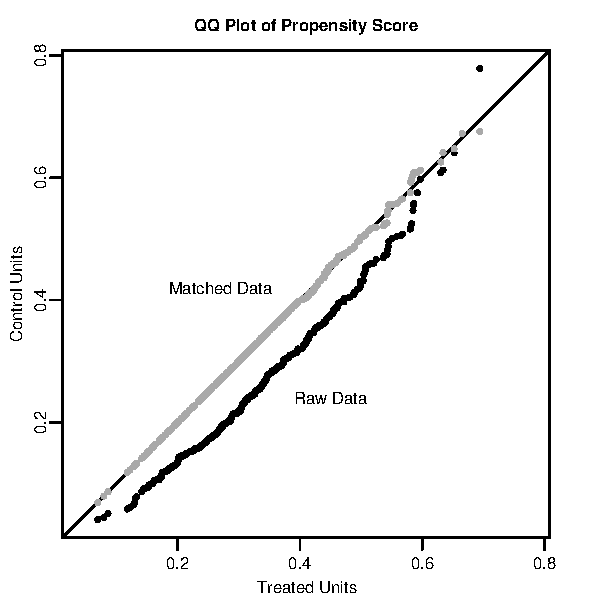
\includegraphics[height=3in,angle=0]{figs/kochqq.pdf}
 \end{center} 
 \vspace{-0.275in}
 \caption{QQ plot of propensity score for candidate visibility. The
   black dots represent empirical QQ estimates for the raw data.  The
   grey dots represent QQ estimates for the matched data.  The
   45-degree line indicates identical distributions.}
 \label{fg:kochQQ}
\end{figure}

The original data include 853 visible Republican male candidates,
compared to only 350 invisible ones.  We therefore redefine the
treatment to examine the impact of being invisible on those 350
candidates.  Through experimentation, we find that propensity score
matching improves balance substantially.  We estimate propensity score
via a logistic regression of visibility on all six pretreatment
covariates.  We conduct an optimal one-to-one nearest neighbor
matching based on the estimated propensity score, resulting in 350
visible candidates matched with 350 invisible candidates.  As
Figure~\ref{fg:kochQQ} demonstrates, matching leads to treatment and
control group values of the estimated propensity score being identical
at almost every quantile, with grey dots lining up along the 45-degree
line.  The percent balance improvement in mean differences is
substantial, ranging at worst from 50.1 percent in the perception of
party ideology to 82.0 percent in respondent ideology, and at best to
94.5--99.9 for the remaining covariates.

With this preprocessed data set we can now run the comparable least
squares analysis as in \citet{Koch02}.  The only difference is that we
run the analysis for the matched dataset.  This analysis yields an
estimated average treatment effect of $-0.03$ with an estimated
standard error of $0.07$, suggesting that there is not much of an
effect of invisibility on Republican male candidates.

We now turn to our main (methodological) purpose of evaluating model
sensitivity by studying the variance of causal effect point estimates
for 63 (=$\sum_{i=1}^6 {6 \choose i}$) regressions containing all
possible subsets of Koch's six covariates, again for simplicity
restricting ourselves to only permutations of the possible main
effects.  We thereby estimate 63 separate point estimates for the raw
and for the preprocessed data.

Figure~\ref{fg:kochdens} plots densities of the ATTs from the raw and
preprocessed data.  As expected, estimates are much less variable in
the preprocessed data.  Estimated effects from the raw data (see the
dashed line) range from $-0.72$ to $0.11$, signifying that the
invisibility for male candidates has no predictable effect on whether
voters perceive candidates as more liberal.  The point estimate from
the raw data (or any one point estimate) cannot represent the enormous
variability in these results.  Estimates from the preprocessed data
stand in stark contrast to the estimates from the raw data.  The
variability of coefficient estimates is substantially smaller, ranging
from $-0.38$ to $-0.28$, every one of which indicates that not having
visibility reduces voters perceptions of the candidates as liberal.
More importantly from our perspective, the standard deviation across
specifications of the raw data is 10.7 times as large as for the
preprocessed data.
\begin{figure}[t] 
 \begin{center}
   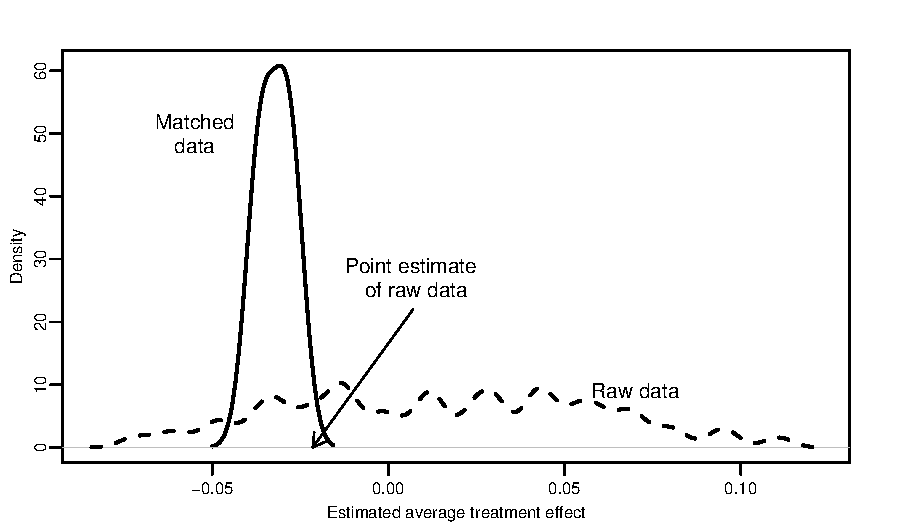
\includegraphics[height=3in,angle=0]{figs/kochdens.pdf}
 \end{center} 
 \vspace{-0.275in}
 \caption{Density estimates of estimated effects of
   being a highly visible female Republican candidate across 63
   possible specifications with the Koch data.  The dashed line
   presents estimates for the raw dataset and the solid line for the
   matched dataset.  The vertical arrow presents the point estimate of
   the regression comparable to the one presented in the original
   paper.  This figure shows that treatment effect estimates are much
   more sensitive to model specification for the raw dataset compared
   to the matched dataset.}
 \label{fg:kochdens}
\end{figure}

\section{What Can Go Wrong}

The advantage of matching is that it is relatively robust to small
changes in procedures, and produces a data set that is by design less
sensitive to modeling assumptions.  However, like any method, using it
badly or to ill effect is certainly possible.  Thus, in this section,
we discuss four ways in which preprocessing can go wrong and how
researchers might try to avoid these problems.

First, since the curse of dimensionality affects balancing
diagnostics, we may well miss a higher dimensional aspect of imbalance
when checking lower dimensional summaries.  Even if we are
uninterested in testing these with our parametric model, they can
affect our estimates.  Such will be the case with parametric models
with or without preprocessing, and so in all but the most unusual
cases preprocessing should at least not make things worse.  One
pathological case where preprocessing could hurt is if some covariate
has a huge effect on the outcome variable and preprocessing slightly
reduces balance on this variable but improves it for all the others.
A researcher might be fooled into choosing a matching tradeoff like
this if he or she were not aware of the large effect of this
covariate.  Carefully evaluating what covariates are likely to have
the largest effects, and using multiple measures of balance, are
essential in avoiding this pitfall.

Second, as with all statistical methods, a bias-variance tradeoff
exists for matching.  If we drop many observations during
preprocessing and balance is not substantially improved, the mean
square error (or other mean-variance summary) might actually increase.
Users must pay close attention to this tradeoff during the process of
matching, but no precise rules exist for how to make these choices.
In particular, the methodological literature offers no formal
estimates of mean square error and so in marginal cases it can be
difficult to know whether or how much preprocessing will help.  Of
course, dropping observations does not necessarily mean that
preprocessing is worse, since improving balance can also increase
efficiency, and in any event including imbalanced observations
requiring extrapolation in a parametric analysis merely produces false
precision.  So although estimated standard errors may increase in some
cases with preprocessing, they would likely be more accurate.
Moreover, in many situations, eliminating observations far from the
rest of the data as matching does will reduce heterogeneity and
thereby further reduces the variance.

Third, the matching literature offers a large number of possible and
seemingly ad hoc procedures.  From one perspective, we might be
concerned about the sensitivity of our results to changes in this
process, just as we have been concerned with the sensitivity of causal
effect estimates to parametric modeling assumptions.  This is not
normally viewed as a major issue since the right procedure is the one
that maximizes balance (with $n$ as large as possible), no matter how
many procedures we try.  By applying this criterion in a disciplined
way (i.e., without consulting $y$) to a large number of possible
matching procedures, no choices are open to the analyst.  Instead,
researchers should merely run as many as possible and choose by this
procedure.  Unlike parametric modeling exercises, we need not choose
this matching procedure or another; we merely run as many as feasible,
or likely to reduce bias and model dependence, and apply this
criterion.

Finally, by dropping observations, we may wind up losing some
critically important cases or may change either the information base
of our sample or, in special cases such as when dropping treated
units, the definition of causal effect.  Examining the dropped cases
provides an easy diagnostic for this problem.  However, we must be
alert to the problem that if we learn that some critical units are
dropped, then it may mean that no appropriate matches can be found for
them.  In this situation, we may be forced to conclude that the data
do not contain sufficient information to answer the questions posed,
no matter what method is chosen.

\section{Concluding Remarks}

Anyone using a parametric statistical technique for long enough (and
it doesn't take very long) will recognize the difficulty of choosing
which of hundreds of possible regressions to present in a written
work.  This choice is difficult, fraught with ethical and
methodological dilemmas, and not covered in any serious way in
classical statistics texts.  Parametric methods merely assume that we
know the correct specification.  In practice, the ``correct''
specification is chosen after looking at the estimates and so it is
never clear to a reader whether an article is a true test of an ex
ante hypothesis, in the sense that the author was vulnerable to being
proved wrong, or whether the article is merely a proof of the
existence of at least one specification consistent with the author's
favored hypothesis.  Researchers are often frustrated with how their
key causal estimates depend sensitively on specification decisions
they have not thought about and on which they have few real opinions.

We provide a way around at least part of this problem.  Preprocessing
raw data with the matching procedures we recommend makes familiar
parametric methods a much more reliable tool of empirical analysis
and, in particular, causal effect estimates become far more
insensitive to seemingly arbitrary choices in model specification.  If
we read an article demonstrating that balance has been achieved for a
data set, readers can worry considerably less that slightly different
specifications than those discussed in the text will greatly alter its
empirical conclusions.  Analysts using preprocessing have two chances
to get their analysis right, in that if either the matching procedure
or the subsequent parametric analysis is specified correctly (and even
if one of the two is incorrectly specified), causal estimates will
still be consistent.

Alternative approaches to reducing model dependence include
cross-validation \citep{BlaSmi04}, weighting \citep{RobRot03,
  HirImbRid03}, nonparametric techniques, robust estimation, and
fitting checks for parametric models.  Although when used properly
each of these approaches reduce model dependence, matching is simpler
to use and understand, and would work without modification to improve
all the parametric models now used in the social sciences.  Matching
even works well with these ``alternative'' approaches.

\appendix
\section{Matching Software}\label{s:matchit}

A variety of excellent software is available to perform matching
\citep{AbaDruLeb02, BecIch02, BerKos03, Hansen05, LeuSia04, Parsons00,
  Parsons01, Sekhon04}.  However, each program implements only a
specialized subset of available statistical procedures.  Moreover,
they are spread over a range of different languages and packages,
which would normally make it impractical to use more than one for any
applied project.  Thus, as a companion to and in the same spirit as
this paper, we have written software (called MatchIt, available at
\url{http://gking.harvard.edu/matchit})  that implements the vast majority of the matching
procedures suggested in the diverse scholarly literatures on this
subject.  Where possible, MatchIt builds on and incorporates existing
packages and, across all the specialized techniques, MatchIt offers a
single, simple, and unified syntax.  Adding procedures to MatchIt is
also easy.

MatchIt operates with a single command that takes an existing dataset
and produces as output a single preprocessed matched dataset.  The
preprocessed dataset can then be used by standard parametric software
just as one would have used the original dataset.  MatchIt also works
seamlessly with the general-purpose statistics program, Zelig
(\citealt{ImaKinLau04}), so that output from MatchIt can be fed into
Zelig without any extra steps.  MatchIt and Zelig are freely available
and run under many operating systems via the open-source and free
statistical program R.

\baselineskip=0.637\baselineskip 
\bibliographystyle{apsr}
\bibliography{gk,gkpubs}

\end{document}
